\documentclass{article}

\usepackage[english]{babel} 
\usepackage[utf8]{inputenc}

\usepackage{amsfonts}
\usepackage{amsmath}
\usepackage{amssymb}
\usepackage{amsthm}
\usepackage[hidelinks]{hyperref}
\usepackage[capitalize]{cleveref}

\usepackage{graphicx}
\usepackage{tikz}
\usepackage[a4paper, total={6in, 8in}]{geometry}

\newtheorem{thm}{Theorem}[section]
\newtheorem{lem}[thm]{Lemma}
\newtheorem{cor}[thm]{Corollary}
\newtheorem{prop}[thm]{Proposition}

\theoremstyle{definition}
\newtheorem{defi}[thm]{Definition}
\newtheorem{exa}[thm]{Example}
\newtheorem{exer}[thm]{Exercise}

\theoremstyle{remark}
\newtheorem{rem}[thm]{Remark}
\newtheorem*{war}{Warning}

\newcommand{\N}{\mathbb N}
\newcommand{\Z}{\mathbb Z}
\newcommand{\Q}{\mathbb Q}
\newcommand{\R}{\mathbb R}
\newcommand{\C}{\mathbb C}

\numberwithin{figure}{section}
\DeclareMathOperator*{\bigast}{\vcenter{\hbox{\Huge$\ast$}}}

\usepackage{tikz-3dplot}
\usepackage{tikz-cd}
\usetikzlibrary{decorations.markings}
\tikzset{
	mid arrow/.style={postaction={decorate,decoration={
	        markings,
	        mark=at position .5 with {\arrow[#1]{stealth}}
		}}},
	double mid arrow/.style={postaction={decorate,decoration={
			markings,
			mark=at position .475 with {\arrow[#1]{stealth}},
			mark=at position .525 with {\arrow[#1]{stealth}}
		}}},
	double mid arrow close/.style={postaction={decorate,decoration={
			markings,
			mark=at position .49 with {\arrow[#1]{stealth}},
			mark=at position .51 with {\arrow[#1]{stealth}}
		}}},
	double mid arrow wide/.style={postaction={decorate,decoration={
			markings,
			mark=at position .45 with {\arrow[#1]{stealth}},
			mark=at position .55 with {\arrow[#1]{stealth}}
		}}},
	double mid arrow closeish/.style={postaction={decorate,decoration={
			markings,
			mark=at position .485 with {\arrow[#1]{stealth}},
			mark=at position .515 with {\arrow[#1]{stealth}}
		}}}
}

\title{Algebraic Topology}
\author{Jack Haviland}
\date{PROMYS Summer 2021}

\begin{document}

\maketitle
\abstract{We rigorously define the fundamental group $\pi_1$, outline some of the most important techniques used to compute $\pi_1$ with worked examples, and discuss the relationship between covering spaces and subgroups of $\pi_1$. The material in the Sections~\ref{sec:van Kampen} and \ref{sec:homotopy} should be skimmed during a first reading in order to understand the definitions and main results, which are applied in \cref{sec:examples}. Note that the treatment of covering spaces moves more quickly than the first two sections and is intdended to be more conceptual. For this reason, some details and/or proofs are omitted.}
\tableofcontents
\newpage

\section{Defining the Fundamental Group}
The goal of algebraic topology is to tell topological spaces apart. We know that two topological spaces are the same when there is a homeomorphism between them. However, it's much harder to tell when two topological spaces are different. For instance, it's (relatively) clear that the cube and the sphere are topologically the same, but what about the torus?

\begin{figure}[h]
	\centering
	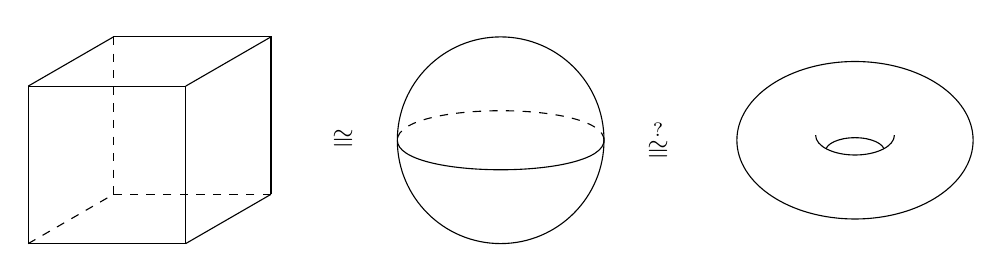
\begin{tikzpicture}
		\draw (-1,-1) rectangle (1,1);
		\draw (-1,1) to node[pos=1] (a) {} +(30:1.25);
		\draw (1,1) to node[pos=1] (b) {} +(30:1.25);
		\draw (1,-1) to node[pos=1] (c) {} +(30:1.25);
		\draw (a.center) to (b.center) to (c.center);
		\draw[dashed] (-1,-1) to node[pos=1] (d) {} +(30:1.25);
		\draw[dashed] (a.center) to (d.center);
		\draw[dashed] (c.center) to (d.center);
		
		\node at (3,0.3125) {$\cong$};
		
		\draw (5,0.3125) circle (1.3125);
		\draw (5 + 1.3125,0.3125) .. controls +(0,-0.5) and +(0,-0.5) .. (5 - 1.3125,0.3125);
		\draw[dashed] (5 + 1.3125,0.3125) .. controls +(0,0.5) and +(0,0.5) .. (5 - 1.3125,0.3125);
		
		\node at (7,0.3125) {$\overset{?}{\cong}$};
		
		\draw (9.5,0.3125) ellipse (1.5 and 1);
		\begin{scope}
			\clip (8.5,0) rectangle (10.5,0.375);
			\draw (9.5,0.375) ellipse (0.5 and 0.25);
		\end{scope}
		
		\begin{scope}
			\clip (9.5,0.375) ellipse (0.5 and 0.25);
			\draw (9.5,0.1725) ellipse (0.375 and 0.1725);
		\end{scope}
	\end{tikzpicture}
	\caption{Some topological spaces}
	\label{fig:topex-2d}
\end{figure}

What about a circle and two tangent circles?

\begin{figure}[h]
	\centering
	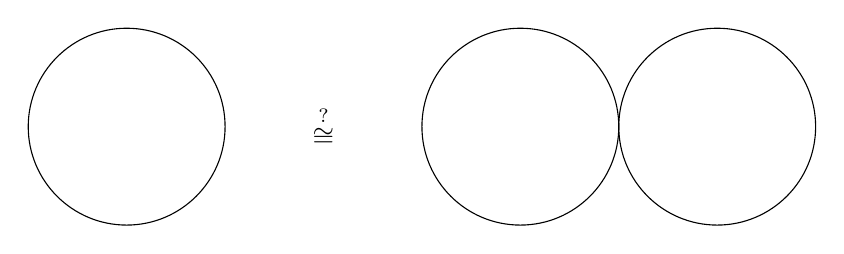
\begin{tikzpicture}
		\draw (0,0) circle (1.25);
		\node at (2.5,0) {$\overset{?}{\cong}$};
		\draw (5,0) circle (1.25);
		\draw (7.5,0) circle (1.25);
	\end{tikzpicture}
	\caption{More topological spaces}
	\label{fig:topex-1d}
\end{figure}

It seems like these should be genuinely different topological spaces, but it's not clear how to prove it. Intuitively, the reason these spaces are different is that they have different numbers of holes. Of course, this begs the question ``what is a hole?'' or ``how do we detect a hole?''.

The second question is more useful in talking about the fundamental group, and the answer is loops. A \emph{loop} is a path, i.e., a map $\gamma : [0, 1] \to X$, such that the endpoints of $\gamma$ are equal, i.e., $\gamma(0) = \gamma(1)$. In $\R^2$, all loops are in some sense boring --- we can just contract a loop down to a single point as in \cref{fig:contracting loop}. However, in $\R^2 \setminus \{0\}$, any loop around the missing point cannot be contracted because the loop would have to pass over the missing point.

\begin{figure}[h]
	\centering
	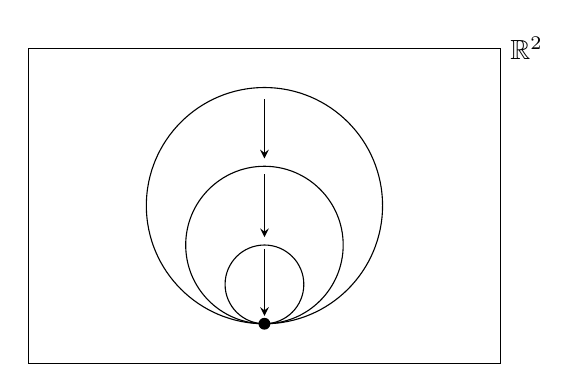
\begin{tikzpicture}
		\foreach \l in {1.5,1,0.5} {
			\draw (0,0) arc (-90:270:\l);
			\draw[-stealth] (90:1.9*\l) -- (90:2*\l - 0.9);
		}
		\fill (0,0) circle (0.075);
		\draw (-3,-0.5) rectangle (3,3.5);
		\node[right] at (3,3.5) {$\R^2$};
	\end{tikzpicture}
	\caption{Contracting a loop to a single point}
	\label{fig:contracting loop}
\end{figure}

\medskip\noindent
\textbf{Notation, Assumptions.} Since we are going to talk about paths a lot, we will write $I = [0, 1] \subseteq \R$ for the closed unit interval. All spaces are topological spaces and all maps are continuous.

\subsection{Path-Homotopy}
Recall that if $X$ is a space and $x, y \in X$, then a path from $x$ to $y$ is a map $p : I \to X$ with $p(0) = x$ and $p(1) = y$.

\begin{defi}
	Let $p, q : I \to X$ be paths such that $p(0) = q(0)$ and $p(1) = q(1)$. A \emph{path-homotopy} from $p$ to $q$ is a family of paths $H_t$, where $t$ ranges over $I$, such that $H_t$ is always a path from $p(0)$ to $p(1)$, $H_0 = p$, and $H_1 = q$. If there is a path-homotopy from $p$ to $q$, we write $p \simeq q$ and say $p$ and $q$ are path-homotopic.
	
	More formally, a path-homotopy is a map $H : I \times I \to X$, written $H(t, s) = H_t(s)$ (so $s \mapsto H_t(s)$ is a path), such that $H_0 = p$, $H_1 = q$, and for all $t \in I$,
	\[
	H_t(0) = p(0) = q(0)
	\]
	and
	\[
	H_t(1) = p(1) = q(1).
	\]
	That is, for all $t$, $H_t$ is a path from $p(0)$ to $p(1)$.
\end{defi}

We think of a path-homotopy as continuously deforming $p$ into $q$ via intermediate paths $H_t$. Another equivalent definition is that $t \mapsto H_t$ is a path from $p$ to $q$ in the space of paths in $X$.

\begin{figure}[h]
	\centering
	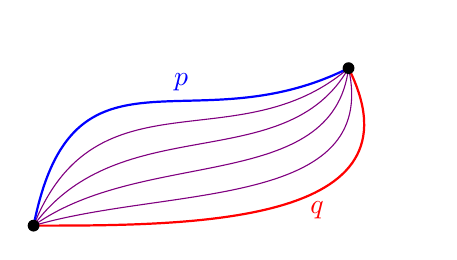
\begin{tikzpicture}
%		\draw (-0.5,-0.25) rectangle (4.5,2.25);
		\foreach \t in {0.2,0.4,0.6,0.8} {
			\draw[violet] (0,0) .. controls +(\t*0.5 + 2 - \t*2,\t*2.5) and +(\t*-2 + 1 - \t,\t*-1 + -2 - \t*-2) .. (4,2);
		}
		
		\draw[thick, blue] (0,0) .. controls +(0.5,2.5) and +(-2,-1) .. (4,2) node[pos=0.6, above] {$p$};
		
		\draw[thick, red] (0,0) .. controls +(2,0) and +(1,-2) .. (4,2) node[pos=0.6, below] {$q$};
		
		\fill (0,0) circle (0.075);
		\fill (4,2) circle (0.075);
	\end{tikzpicture}
	\caption{Path-homotopy as intermediate paths deforming $p$ to $q$}
	\label{fig:path-homotopy visual}
\end{figure}

\color{red}
\begin{war}
	We have only defined path-homotopy for pairs of paths between the same points. It is possible, and interesting, to define a more general kind of homotopy, but this makes things uninteresting in the case of paths because all paths are homotopic (at least in a path-connected space).
\end{war}
\color{black}

\begin{exa}
	The \emph{straight line homotopy} in $\R^n$: if $p, q : I \to \R^n$ are paths from $x$ to $y$, define
	\[
	H_t(s) = (1 - t)p(s) + tq(s).
	\]
	Then
	\begin{align*}
		H_t(0) &= (1 - t)p(0) + tq(0) = (1 - t)x + tx = x\\
		H_t(1) &= (1 - t)p(1) + tq(1) = (1 - t)y + ty = y\\
		H_0(s) &= (1 - 0)p(s) + 0q(s) = p(s)\\
		H_1(s) &= (1 - 1)p(s) + 1q(s) = q(s).
	\end{align*}
	Hence $H_t$ is a path-homotopy from $p$ to $q$. This proves that all paths in $\R^n$ between the same two points are path-homotopic.
	
	Less formally, this homotopy drags each point $p(s)$ along the straight line segment to $q(s)$, which means it works in any convex region of $\R^n$.
	\begin{figure}[h]
	\centering
	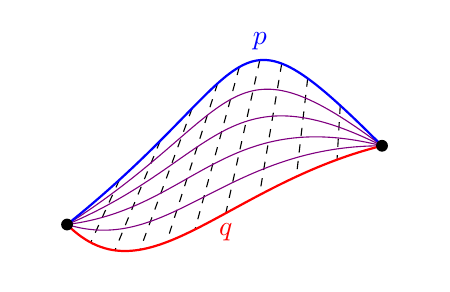
\begin{tikzpicture}
		\useasboundingbox (-0.5,0.5) rectangle (4.5,3.5);
		\path (0,1) .. controls +(2.5,2) and +(-2,2) .. (4,2)
			\foreach \s in {1,...,9} {node[pos=0.\s] (p\s) {}};

		\path (0,1) .. controls +(1,-1) and +(-2,-0.5) .. (4,2)
			\foreach \s in {1,...,9} {node[pos=0.\s] (q\s) {}};
		
		\foreach \s in {1,...,9} \draw[dashed] (p\s.center) -- (q\s.center);
		
		\foreach \t in {0.2,0.4,0.6,0.8} {
			\draw[violet] (0,1) .. controls +(\t*2.5 + 1 - \t*1,\t*2 + -1 - \t*-1) and +(\t*-2 + -2 - \t*-2,\t*2 + -0.5 - \t*-0.5) .. (4,2);
		} 
		
		\draw[thick, blue] (0,1) .. controls +(2.5,2) and +(-2,2) .. (4,2) node[pos=0.6, above] {$p$};
		
		\draw[thick, red] (0,1) .. controls +(1,-1) and +(-2,-0.5) .. (4,2) node[pos=0.6, below] {$q$};
		
		\fill (0,1) circle (0.075);
		\fill (4,2) circle (0.075);
	\end{tikzpicture}
	\caption{Straight line homotopy in $\R^n$ ($n = 2$)}
	\label{fig:straight line homotopy}
\end{figure}
\end{exa}

\begin{exa}
	In $\R^2 \setminus \{0\}$, two paths on different sides of the missing point are not homotopic. This is becuase we can't go ``around'' the missing point, and we can't deform either path through the middle. This is a bit tricky to formalize, so we will leave the rigor for later.
	\begin{figure}[h]
		\centering
		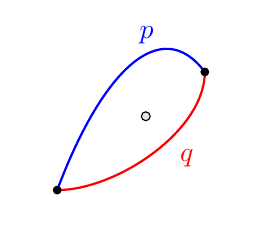
\begin{tikzpicture}[scale=0.75]
			\useasboundingbox (-2,-1.5) rectangle (1.5,1.5);
			\fill[gray!20] (0,0) circle (0.075);
			\draw (0,0) circle (0.075);
			\draw[thick, blue] (-1.5,-1.25) .. controls +(0.75,2) and +(-0.75,1) .. (1,0.75) node[above, pos=0.6] {$p$};
			\draw[thick, red] (-1.5,-1.25) .. controls +(1,0) and +(0,-1) .. (1,0.75) node[below right, pos=0.6] {$q$};
			\fill (-1.5,-1.25) circle (0.075);
			\fill (1,0.75) circle (0.075);
		\end{tikzpicture}
		\caption{Two non-path-homotopic paths around the missing point in $\R^2 \setminus \{0\}$}
		\label{fig:non-homotopic paths}
	\end{figure}
\end{exa}

Our original motivation for path-homotopies was defining a notion of equivalent paths, since we want to measure distinct loops in a space. So, it would be a good idea to check that $\simeq$ makes a good notion of equivalence.

\begin{prop}
	Path-homotopy is an equivalence relation.
\end{prop}

\begin{proof}
	Let $p, q, r : I \to X$ be paths from $x$ to $y$. Then $p \simeq p$ via the path-homotopy $H_t = p$ for all $t$. If $p \simeq q$ via a path-homotopy $H_t$, define $H'_t = H_{1 - t}$; this show $q \simeq p$ because
	\begin{align*}
		H'_0 &= H_1 = q,\\
		H'_1 &= H_0 = p,\\
		H'_t(0) &= H_{1 - t}(0) = x,\\
		H'_t(1) &= H_{1 - t}(1) = y
	\end{align*}
	for all $t$. Finally, if $p \simeq q$ and $q \simeq r$ via path-homotopies $F_t$ and $G_t$, respectively, define
	\[
	H_t = \begin{cases}
		F_{2t} & \text{if } t \leq 1/2\\
		G_{2t - 1} & \text{if } t \geq 1/2,
	\end{cases}
	\]
	which is well-defined because $F_1 = G_0 = q$. Then
	\begin{align*}
		H_0 &= F_0 = p,\\
		H_1 &= G_1 = r,\\
		H_t(0) &= \begin{cases}
			F_{2t}(0) = x\\
			G_{2t - 1}(0) = x,
		\end{cases}\\
		H_t(1) &= \begin{cases}
			F_{2t}(1) = y\\
			G_{2t - 1}(1) = y
		\end{cases}
	\end{align*}
	for all $t$. Hence $p \simeq r$.
\end{proof}

For the last step in this proof, all we are doing is performing the homotopy from $p$ to $q$ first, then from $q$ to $r$, both at twice the original speed. Visually, this looks like the usual family of maps interpolating between $p$ and $r$, but with $q$ directly in the middle (see \cref{fig:transitive homotopies}).

\begin{figure}[h]
	\centering
	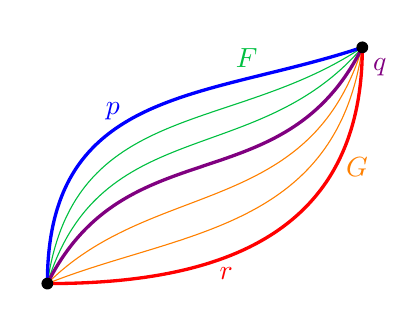
\begin{tikzpicture}
		\useasboundingbox (-0.25, -0.25) rectangle (4.25,3.25);
		\foreach \t in {1/3,2/3} {
			\draw[green!75!blue] (0,0) .. controls +(1 - \t, \t*2.5 + 2 - \t*2) and +(\t*-2 + -1 - \t*-1, \t*-2/3 + -2 - \t*-2) .. (4,3);
		}
		
		\foreach \t in {1/3,2/3} {
			\draw[orange] (0,0) .. controls +(\t + 2 - \t*2, \t*2) and +(\t*-1, \t*-2 + -2.5 - \t*-2.5) .. (4,3);
		}
		
		\draw[very thick, blue] (0,0) .. controls +(0,2.5) and +(-2,-2/3) .. (4,3) node[above, pos=0.4] {$p$} node[above, pos=0.75, green!75!blue] {$F$};
		\draw[very thick, violet] (0,0) .. controls +(1,2) and +(-1,-2) .. (4,3) node[below right, pos=1] {$q$};
		\draw[very thick, red] (0,0) .. controls +(2,0) and +(0,-2.5) .. (4,3) node[below, pos=0.4] {$r$} node[right, pos=0.75, orange] {$G$};
		
		\fill (0,0) circle (0.075);
		\fill (4,3) circle (0.075);
	\end{tikzpicture}
	\caption{Performing two path-homotopies at once}
	\label{fig:transitive homotopies}
\end{figure}

\subsection{Defining $\pi_1$}
\subsubsection{Fundamental group as a set}
We are now ready to define the fundamental group, at least as a set. Hopefully, the definition will not come as a surprise because of everything we have already done. We will have to do some work to define and justify a group structure and we could do the work beforehand, but it is better motivated once we know what kind of objects we are working with.

Recall that a loop in a space $X$ based at a point $x_0 \in X$ is a path in $X$ whose endpoints are both $x_0$.

\begin{defi}
	Let $X$ be a space and $x_0 \in X$. The \emph{fundamental group} of $X$ based at $x_0$, denoted $\pi_1(X, x_0)$, is the set of path-homotopy classes of loops based at $x_0$. That is,
	\[
	\pi_1(X, x_0) = \frac{\{\gamma : I \to X \mid \gamma(0) = \gamma(1) = x_0\}}{\simeq}.
	\]
	The elements of $\pi_1(X, x_0)$ are written $[\gamma]$, where $\gamma$ is a loop in $X$ based at $x_0$.
\end{defi}

\color{red}
\begin{war}
	The base point $x_0$ is really important in this definition. For example, consider the disjoint union of a disc with a $2$-torus. As we have shown, there are no nontrivial loops in the disc, which is a convex subset of $\R^2$. On the other hand, although we have not shown this rigorously, there are at least two distinct kinds of nontrivial loops in the torus.
\end{war}
\color{black}
	
Note, however, that if $X$ is path connected, then $\pi_1(X, x_0) \cong \pi_1(X, x_1)$ for all $x_0, x_1 \in X$, which can be proved using ``change of basepoint'' maps induced by a path between the points $x_0$ and $x_1$. So in this case it makes sense to talk about $\pi_1(X)$ as an abstract group up to isomorphism, but to work with elements of the fundamental group we still need to fix a base point.

Now that we have $\pi_1(X, x_0)$ as a set, we need to define a group operation. The most natural way to combine paths is to connect them at their endpoints. This is called \emph{composition of paths}, which is a terrible name because it has nothing to do with function compoosition even though paths are functions. Since we don't want to move the endpoints of our paths, we will only compose paths whose endpoints are already compatible.

\begin{defi}
	Let $p, q : I \to X$ be paths with $p(1) = q(0)$. Define $p * q : I \to X$ by
	\[
	p * q(s) = \begin{cases}
		p(2s) & \text{if } s \leq 1/2\\
		q(2s - 1) & \text{if } s \geq 1/2.
	\end{cases}
	\]
\end{defi}

\begin{figure}[h]
	\centering
	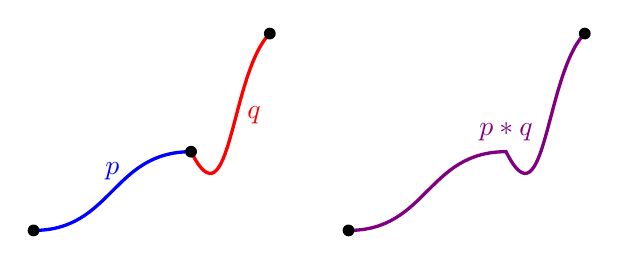
\begin{tikzpicture}
		\draw[very thick, blue] (0,0) .. controls +(1,0) and +(-1,0) .. (2,1) node[midway, above] {$p$};
		\draw[very thick, red] (2,1) .. controls +(0.5,-1) and +(-0.5,-0.5) .. (3,2.5) node[pos=0.6, right] {$q$};
		\fill (0,0) circle (0.075);
		\fill (2,1) circle (0.075);
		\fill (3,2.5) circle (0.075);
		
		\begin{scope}[shift={(4,0)}]
			\draw[very thick, violet] (0,0) .. controls +(1,0) and +(-1,0) .. (2,1) node[pos=1, above] {$p * q$} .. controls +(0.5,-1) and +(-0.5,-0.5) .. (3,2.5);
			\fill (0,0) circle (0.075);
			\fill (3,2.5) circle (0.075);
		\end{scope}
	\end{tikzpicture}
	\caption{Composition of compatible paths}
	\label{fig:path composing}
\end{figure}

The composition of loops with the same basepoint is always defined, so composition of paths induces an operation on $\pi_1(X, x_0)$. Specifically, for elements $[\alpha], [\beta] \in \pi_1(X, x_0)$, define
\[
[\alpha] * [\beta] = [\alpha * \beta].
\]
We need to show that this operation is well-defined on path-homotopy classes. If $\alpha \simeq \alpha'$ and $\beta \simeq \beta'$ via path-homotopies $F_t$ and $G_t$, then $H_t = F_t * G_t$ is a path-homotopy from $\alpha * \beta$ to $\alpha' * \beta'$:
\begin{align*}
	H_0 &= F_0 * G_0 = \alpha * \beta\\
	H_1 &= F_1 * G_1 = \alpha' * \beta'\\
	H_t(0) &= F_t * G_t(0) = F_t(0) = x_0\\
	H_t(1) &= F_t * G_t(1) = G_t(1) = x_0
\end{align*}
because $F_t$ and $G_t$ are always paths based at $x_0$. Hence $\alpha * \beta \simeq \alpha' * \beta'$, proving that $*$ is well-defined on path-homotopy classes.

\subsubsection{Proving group axioms}
We now devote ourselves to proving the following theorem.

\begin{thm}
	If $X$ is a space and $x_0 \in X$, then $\pi_1(X, x_0)$ is a group with respect to composition of paths.
\end{thm}

We need to show associativity, existence of an identity, and existence of inverses. To do this, it will be very convenient to understand reparametrizations of paths: if $j : I \to I$ is map which fixes $0$ and $1$ and $p : I \to X$ is a path in $X$, we say $p \circ j$ is a \emph{reparametrization} of $p$. A good way to think of a reparametrization is changing the speed of a path.

\begin{lem}\label{lem:reparametrization}
	Reparametrizing a path does not change its path-homotopy class.
\end{lem}

\begin{proof}
	Let $p : I \to X$ be a path and $j : I \to I$ a map fixing $0$ and $1$. With the straight-line homotopy, we know $j$ is path-homotopic to the identity map $\mathrm{id}_I : I \to I$, so let $H_t$ be a path-homotopy showing $j \simeq \mathrm{id}_I$. Define $H'_t = p \circ H_t$. Then
	\begin{align*}
		H'_0 &= p \circ H_0 = p \circ j\\
		H'_1 &= p \circ H_1 = p \circ \mathrm{id}_I\\
		H'_t(0) &= p \circ H_t(0) = p(0)\\
		H'_t(1) &= p \circ H_t(1) = p(1)
	\end{align*}
	because $j$ and $\mathrm{id}_I$ both fix the endpoints $0$ and $1$, so $H_t(0) = 0$ and $H_t(1) = 1$ for all $t$. Hence $H'_t$ is a path-homotopy showing $p \circ j \simeq p$.
\end{proof}

Now, we can prove associativity and identity much more easily. For associativity, if $[\alpha], [\beta], [\gamma] \in \pi_1(X, x_0)$, then $\alpha * (\beta * \gamma)$ is a reparametrization of $(\alpha * \beta) * \gamma$. Specifically, in $\alpha * (\beta * \gamma)$, we first go $2$ times faster through $\alpha$, then $4$ times faster through $\beta$ and $\gamma$. On the other hand, in $(\alpha * \beta) * \gamma$, we first go $4$ times faster through $\alpha$ and $\beta$, then $2$ times faster through $\gamma$. Since the order in which the loops appear is the same, to get from $\alpha * (\beta * \gamma)$ to $(\alpha * \beta) * \gamma$ we just need to speed $\alpha$ up and slow $\gamma$ down. For completeness sake, here is a map $j : I \to I$ such that $\alpha * (\beta * \gamma) \circ j = (\alpha * \beta) * \gamma$:
\[
j(s) = \begin{cases}
	2s & \text{if } s \leq 1/4\\
	s + 1/4 & \text{if } 1/4 \leq s \leq 1/2\\
	s/2 + 1/2 & \text{if } 1/2 \leq s.
\end{cases}
\]
The details of checking this are at best a good thought experiment and at worst a waste of time; the visual in \cref{fig:reparam visual} is likely to be much more enlightening. Since this shows $\alpha * (\beta * \gamma)$ is a reparametrization of $(\alpha * \beta) * \gamma$, it follows from \cref{lem:reparametrization} that $[\alpha * (\beta * \gamma)] = [(\alpha * \beta) * \gamma]$. Hence associativity holds in $\pi_1(X, x_0)$.

\begin{figure}[h]
	\centering
	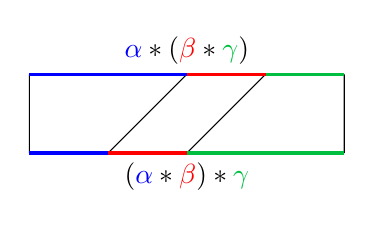
\begin{tikzpicture}
		\draw (0,0) -- (0,-1)
			  (2,0) -- (1,-1)
			  (3,0) -- (2,-1)
			  (4,0) -- (4,-1);
		
		\draw[very thick, blue] (0,0) -- (2,0);
		\draw[very thick, red] (2,0) -- (3,0);
		\draw[very thick, green!75!blue] (3,0) -- (4,0);
		\node[above] at (2,0) {$\color{blue}\alpha\color{black} * (\color{red}\beta\color{black} * \color{green!75!blue}\gamma\color{black})$};
		
		\draw[very thick, blue] (0,-1) -- (1,-1);
		\draw[very thick, red] (1,-1) -- (2,-1);
		\draw[very thick, green!75!blue] (2,-1) -- (4,-1);
		\node[below] at (2,-1) {$(\color{blue}\alpha\color{black} * \color{red}\beta\color{black}) * \color{green!75!blue}\gamma\color{black}$};
	\end{tikzpicture}
	\caption{Associativity of path composition via reparametrization}
	\label{fig:reparam visual}
\end{figure}

Next, we need to verify that there is an identity element in $\pi_1(X, x_0)$. Morally, this should be the constant loop $c$ at $x_0$, since if any loop should be considered trivial it is the constant loop. Indeed, this is the case, since if $[\gamma] \in \pi_1(X, x_0)$, then $\gamma * c$ and $c * \gamma$ are both reparametrizations of $\gamma$. Specifically, $\gamma * c$ corresponds to going through $\gamma$ twice as fast and then stopping at $x_0$ for the remaining time, while $c * \gamma$ corresponds to waiting at $x_0$ for the half the time, then going through $\gamma$ twice as fast. For completeness sake, here is a map $j : I \to I$ such that $\gamma \circ j = \gamma * c$:
\[
j(s) = \begin{cases}
	2s & \text{if } s \leq 1/2\\
	1 & \text{if } s \geq 1/2
\end{cases}
\]
and a map $j' : I \to I$ such that $\gamma \circ j' = c * \gamma$:
\[
j'(s) = \begin{cases}
	0 & \text{if } s \leq 1/2\\
	2s - 1 & \text{if } s \geq 1/2.
\end{cases}
\]
Familiar comments apply about checking the details of these maps; a visualization similar to the visual for associativity appears in \cref{fig:constant is identity}.

\begin{figure}[h]
	\centering
	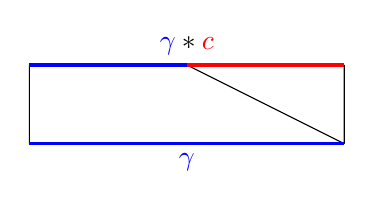
\begin{tikzpicture}
		\draw (0,0) -- (0,-1)
			  (2,0) -- (4,-1)
			  (4,0) -- (4,-1);
		
		\draw[very thick, blue] (0,0) -- (2,0);
		\draw[very thick, red] (2,0) -- (4,0);
		\node[above] at (2,0) {$\color{blue}\gamma\color{black} * \color{red}c\color{black}$};
		
		\draw[very thick, blue] (0,-1) -- (4,-1);
		\node[below] at (2,-1) {$\color{blue}\gamma$};
	\end{tikzpicture}
	\qquad\qquad\qquad
	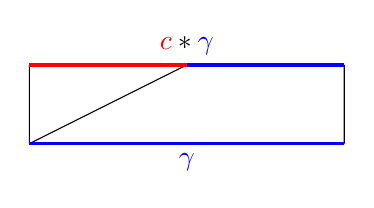
\begin{tikzpicture}
		\draw (0,0) -- (0,-1)
			  (2,0) -- (0,-1)
			  (4,0) -- (4,-1);
		
		\draw[very thick, red] (0,0) -- (2,0);
		\draw[very thick, blue] (2,0) -- (4,0);
		\node[above] at (2,0) {$\color{red}c\color{black} * \color{blue}\gamma\color{black}$};
		
		\draw[very thick, blue] (0,-1) -- (4,-1);
		\node[below] at (2,-1) {$\color{blue}\gamma$};
	\end{tikzpicture}
	\caption{The constant path is a path-composition identity, up to path-homotopy}
	\label{fig:constant is identity}
\end{figure}

Finally, we need to check that inverses exist. Given $[\gamma] \in \pi_1(X, x_0)$, define $\bar\gamma : I \to X$ by $\bar\gamma(s) = \gamma(1 - s)$, so $\bar\gamma$ is just $\gamma$ in reverse. This is a natural candidate for the inverse of $\gamma$, since it ``undoes'' everything $\gamma$ does. To prove this, define $\gamma_t : I \to X$ by
\[
\gamma_t(s) = \begin{cases}
	\gamma(s) & \text{if } s \leq 1 - t\\
	\gamma(t) & \text{if } s \geq 1 - t.
\end{cases}
\]
The idea here is that $\gamma_t$ follows $\gamma$ until time $t$, and then stops. Even though $\gamma_t$ is not a loop at $x_0$, $\gamma_t * \bar\gamma_t$ is, since it follows $\gamma$ to $\gamma(t)$ and then turns around and goes back the way it came.

\begin{figure}[h]
	\centering
	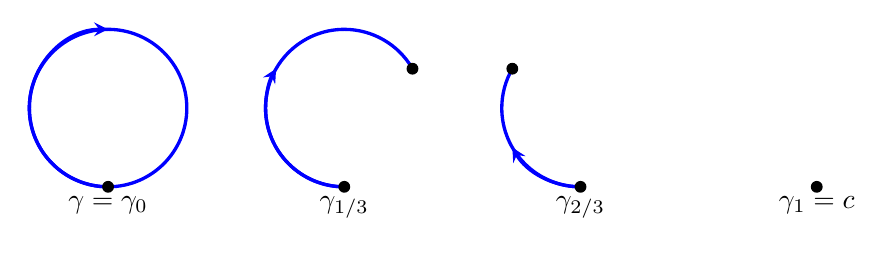
\begin{tikzpicture}
		\begin{scope}[shift={(0,0)}]
			\draw[very thick, blue, -stealth] (0,0) arc (270:90:1);
			\draw[very thick, blue] (0,0) arc (270:-90:1);
			\fill (0,0) circle (0.075);
			\node[below] at (0,0) {$\gamma = \gamma_0$};
		\end{scope}
		
		\begin{scope}[shift={(3,0)}]
			\draw[very thick, blue, -stealth] (0,0) arc (270:150:1);
			\draw[very thick, blue] (0,0) arc (270:30:1);
			\fill (0,0) circle (0.075);
			\fill (30:1) + (0,1) circle (0.075);
			\node[below] at (0,0) {$\gamma_{1/3}$};
		\end{scope}
		
		\begin{scope}[shift={(6,0)}]
			\draw[very thick, blue, -stealth] (0,0) arc (270:210:1);
			\draw[very thick, blue] (0,0) arc (270:150:1);
			\fill (0,0) circle (0.075);
			\fill (150:1) + (0,1) circle (0.075);
			\node[below] at (0,0) {$\gamma_{2/3}$};
		\end{scope}
		
		\fill (9,0) circle (0.075);
		\node[below] at (9,0) {$\gamma_1 = c$};
	\end{tikzpicture}
	\caption{The paths $\gamma_t$}
	\label{fig:inverse visual}
\end{figure}

Now define $H_t = \gamma_t * \bar\gamma_t$, which will be our path-homotopy from $\gamma * \bar\gamma$ to $c$. To see this, note that
\begin{align*}
	H_0 &= \gamma_0 * \bar\gamma_0 = \gamma * \bar\gamma\\
	H_1 &= \gamma_1 * \bar\gamma_1 = c * c = c\\
	H_t(0) &= \gamma_t * \bar\gamma_t(0) = \gamma_t(0) = \gamma(0)\\
	H_t(1) &= \gamma_t * \bar\gamma_t(1) = \bar\gamma_t(1) = \bar\gamma(1) \gamma(0).
\end{align*}
Hence $\gamma * \bar\gamma \simeq c$, so $\bar\gamma * \gamma = \bar\gamma * \bar{\bar\gamma} \simeq c$.

Since we have verified associativity and existence of an identity and inverses, we conclude that $\pi_1(X, x_0)$ is a group under composition of paths.\qed

\subsection{First Examples}
The rest of this section will be devoted to computing fundamental groups for some simple examples, giving less rigorous arguments. In the future, we will look at more concrete computational tools.

\begin{exa}
	For any $x_0 \in \R^n$, $\pi_1(\R^n, x_0) \cong 1$ because all loops based at $x_0$ are path-homotopic. More generally, this holds for any convex subset of $\R^n$.
\end{exa}

\begin{exa}
	For any $n > 1$ and any $x_0 \in S^n$, $\pi_1(S^n, x_0) \cong 1$. We can illustrate the idea for the proof in $S^2$, which is that any loop in $S^n$ bounds a disc and therefore can be pulled tight; see \cref{fig:pi_1 Sn}.
	\begin{figure}[h]
		\centering
		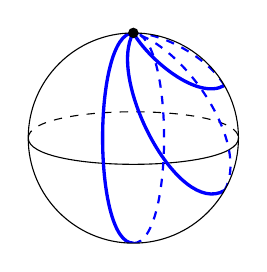
\begin{tikzpicture}[scale=0.89]
			\begin{scope}
				\clip (0,0) circle (1.5);
				
				\draw (-1.5,0) .. controls +(0,-0.5) and +(0,-0.5) .. (1.5,0);
				\draw[dashed] (-1.5,0) .. controls +(0,0.5) and +(0,0.5) .. (1.5,0);
				
				\draw[very thick, blue] (0,-1.5) to[out=180, in=180, looseness=0.5] (0,1.5);
				\draw[thick, dashed, blue] (0,-1.5) to[out=0, in=0, looseness=0.5] (0,1.5);
				
				\draw[very thick, blue] (-30:1.5) to[out=210, in=-120, looseness=0.75] (0,1.5);
				\draw[thick, dashed, blue] (-30:1.5) to[out=60, in=-15, looseness=0.75] (0,1.5);
				
				\draw[very thick, blue] (30:1.5) to[out=210, in=-60, looseness=0.75] (0,1.5);
				\draw[thick, dashed, blue] (30:1.5) to[out=120, in=0, looseness=0.75] (0,1.5);
				
				\draw[-stealth, blue] (-85:1.75) arc (-85:-35:1.75);
				\draw[-stealth, blue] (-25:1.75) arc (-25:25:1.75);
				\draw[-stealth, blue] (35:1.75) arc (35:85:1.75);
			\end{scope}
			
			\draw (0,0) circle (1.5);
			\fill (0,1.5) circle (0.075);
		\end{tikzpicture}
		\caption{A loop in $S^n$ ($n = 2$) being pulled tight}
		\label{fig:pi_1 Sn}
	\end{figure}
\end{exa}

\begin{exa}
	We just saw that for $n > 1$, $\pi_1(S^n, x_0)$ is trivial. What happens when $n = 1$?
	
	A loop in $S^1$ has to ``go around'' the circle some number of times. We want to use this fact to assign a number to each loop, specifically the number of times the loop winds around $S^1$. This was suggestive wording, since this number is often called the \emph{winding number} of the loop, and this assignment will induce an isomorphism $\pi_1(S^1, x_0) \cong \Z$.
	
	To give this map more explicitly, consider the picture in \cref{fig:path lifting S^1}. We can take a path starting at $x_0$ in $S^1$ and lift it to a path in $\R$ by traveling the same distance\footnote{Actually, we want to divide the distance by $2\pi$ so that loops line up with integers.} in $\R$ starting at $x_0$, with clockwise corresponding to positive and counterclockwise negative. Then a loop in $S^1$ corresponds exactly to a path in $\R$ that ends at an integer. Moreover, the composition of two paths corresponds to the path ending at the sum of the corresponding endpoints, so we have constructed a group homomorphim.
	
	Conversely, given a path in $\R$ ending at an integer, we can project the path down onto $S^1$ by wrapping it around the circle. By construction, this is the inverse of our lifting map, so we have constructed an isomorphism showing $\pi_1(S^1, x_0) \cong \Z$.
	
	\begin{figure}[h]
		\centering
		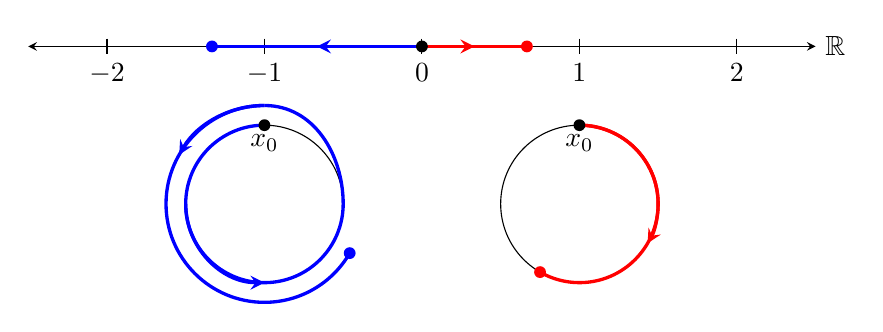
\begin{tikzpicture}
			\draw[stealth-stealth] (-5,0) -- (5,0);
			\node[right] at (5,0) {$\R$};
			\foreach \x in {-2,...,2} {
				\draw (2*\x,0.1) -- (2*\x,-0.1);
				\node[below] at (2*\x,-0.1) {$\x$};
			}
			
			\begin{scope}[shift={(2,0)}]
				\draw (0,-2) circle (1);
				
				\draw[very thick, -stealth, red] (0,-1) arc (90:-30:1);
				\draw[very thick, red] (0,-1) arc (90:-120:1);
				\fill[red] (-120:1) + (0,-2) circle (0.075);
				
				\fill (0,-1) circle (0.075);
				\node[below] at (0,-1) {$x_0$};
			\end{scope}
			\draw[very thick, -stealth, red] (0,0) -- (2/3,0);
			\draw[very thick, red] (0,0) -- (4/3, 0);
			\fill[red] (4/3,0) circle (0.075);
			
			\begin{scope}[shift={(-2,0)}]
				\draw (0,-2) circle (1);
				
				\draw[very thick, -stealth, blue] (-1,-2) arc (180:270:1);
				\draw[very thick, blue] (0,-1) arc (90:360:1);
				\draw[very thick, blue] (1,-2) to[out=90, in=0] (0,-0.75);
				\draw[very thick, blue] (0,-0.75) arc (90:330:1.25);
				\draw[very thick, -stealth, blue] (0,-0.75) arc (90:150:1.25);
				\fill[blue] (330:1.25) + (0,-2) circle (0.075);
				
				\fill (0,-1) circle (0.075);
				\node[below] at (0,-1) {$x_0$};
			\end{scope}
			\draw[very thick, -stealth, blue] (0,0) -- (-4/3,0);
			\draw[very thick, blue] (0,0) -- (-8/3, 0);
			\fill[blue] (-8/3,0) circle (0.075);
			
			\fill (0,0) circle (0.075);
		\end{tikzpicture}
		\caption{Lifting paths from $S^1$ to $\R$.}
		\label{fig:path lifting S^1}
	\end{figure}
\end{exa}

\subsection*{Exercises}
\begin{enumerate}
	\item A subset $S \subseteq \R^n$ is called \emph{star-shaped} if there is a point $x_0 \in S$ such that for all $y \in S$, the line segment from $x_0$ to $y$ is contained in $S$. Prove $\pi_1(S, x_0)$ is trivial.
	
	\item Let $f : X \to Y$, $f(x_0) = y_0$. Define $f_* : \pi_1(X, x_0) \to \pi_1(Y, y_0)$ in a natural way and prove your construction is a group homomorphism.
	
	\item Prove that $\pi_1$ is invariant under homeomorphisms. That is, if there is a homeomorphism $f : X \to Y$, then $\pi_1(X, x_0) \cong \pi_1(Y, f(x_0))$.
	
	\item Prove $\pi_1(X \times Y, (x_0, y_0)) \cong \pi_1(X, x_0) \times \pi_1(Y, y_0)$. (\emph{Hint}\footnote{\raisebox{0.25em}{\rotatebox{180}{Consider the map that takes $[\gamma]$ to $([\gamma_X], [\gamma_y])$, where $\gamma(s) = (\gamma_X(s), \gamma_y(s))$.}}})
	
	\item Compute the fundamental group of the $n$-torus $S^1 \times \cdots \times S^1$ ($n$ copies of $S^1$).
\end{enumerate}

\newpage
\section{Computing the Fundamental Group}\label{sec:computing}
Last time, we defined the fundamental group as the set of path-homotopy classes of loops at a basepoint under the operation of path composition and found the fundamental groups of $\pi_1(\R^n, x_0)$ and $\pi_1(S^n, x_0)$. In $\R^n$, we heavily used the vector space structure to define the straight line homotopy. For $S^n$, at least for $n > 2$, we used the idea of contracting any loop around the sphere to a point.

Now, we are going to learn some more general tools to make computing fundamental groups more systematic, rather than coming up with a clever trick every time. There are basically two ideas that we will leverage:
\begin{enumerate}
	\item Breaking spaces down into simpler spaces whose fundamental groups we already understand. This is done using the Seifert-van Kampen theorem.
	\item Deforming spaces in ways that don't affect the fundamental group. These deformations are called \emph{homotopy equivalences}, and we will them and show they preserve the fundmental group.
\end{enumerate}
It is not a bad idea to skim Sections \ref{sec:van Kampen} and \ref{sec:homotopy} to get the statements of \cref{thm:simplified van Kampen} (simplified Seifert-van Kampen) and \cref{cor:homotopy invariance} (homotopy invariance), then move on to the examples during a first read, since the theorems are most important in their applications.

\subsection{The Seifert-van Kampen Theorem}\label{sec:van Kampen}
Let's take another look at one of the examples we considered last time, $\pi_1(S^2, x_0)$. Originally, we said that any loop in $S^2$ is trivial because we can contract any loop to a point around the sphere. Indeed, by taking one point not on the loop out of the sphere, we get an open neighborhood of the loop which is homeomorphic to an open disk, so we can use the straight-line homotopy to contract the loop. However, it would be nice to be able to treat all loops the same way, without having to pick a new open set every time.

We can cover $S^2$ with two disks, the northern and southern hemispheres. Actually, since working with open sets is preferable in this case, we will consider open neighborhoods of the northern and southern hemispheres, whose intersection is an open annulus around the equator. Thus both open sets used in the cover are homeomorphic to an open disk in $\R^2$. We will denote these sets by $N$ and $S$.

If a loop is entirely contained in either $N$ or $S$, as in the blue loop in \cref{fig:covering s^2}, then we can use the straight line homotopy (really, its image under a homeomorphism to $N$ or $S$) to contract the loop. If the loops meanders from one hemisphere to the other, as in the red loop, we need to be a bit more clever.

\begin{figure}[h]
	\centering
	\tdplotsetmaincoords{75}{135}
	\begin{tikzpicture}[scale=3, tdplot_main_coords,opacity=0.0,fill opacity=0.5]
		\tdplotsetpolarplotrange{0}{105}{0}{360};
		\tdplotsphericalsurfaceplot[opacity=0.5]{60}{36}{1}{black}{yellow}{}{}{};
		
		\tdplotsetpolarplotrange{75}{180}{0}{360};
		\tdplotsphericalsurfaceplot[opacity=0.5]{60}{36}{1}{black}{blue}{}{}{};
		
		\draw[opacity=1, very thick, blue!80!black] (120:1) .. controls +(0.5,0,-0.5) and +(0,0.5,0.1) .. (0,0,-1.025);
		\draw[opacity=1, very thick, blue!80!black, dashed] (0,0,-1.025) .. controls +(0,-0.75,-0.15) and +(0,0,1) .. (120:1);
		
		\draw[opacity=1, very thick, red!95!black]
			(120:1) .. controls +(0,0,-0.75) and +(0,0.5,-0.75) .. (0:1) node[midway, below] {$\gamma_1$}
			.. controls +(0,-0.333,0.5) and +(0.1,-0.1,-0.1) .. (1,0,0.92) node[pos=1, above] {$\gamma_2$};
		\draw[opacity=1, very thick, red!95!black, dashed]
			(1,0,0.92) .. controls +(-0.5,0,0.1) and +(0.5,0,-0.25) .. (240:1)
			.. controls +(-0.5,0,0.25) and +(240:0.5) .. (-2,-1,0.15) node[pos=1, above] {$\gamma_3$};
		\draw[opacity=1, very thick, red!95!black]
			(-2,-1,0.15) .. controls +(-0.1,0,-0.1) and +(0,0,0.4) .. (120:1) node[pos=0.85, right] {\large$\gamma$};
		
		\tdplotdrawarc[very thick, opacity=1, -stealth, violet]{(0,0,0)}{1}{120}{60}{}{};
		\tdplotdrawarc[very thick, opacity=1, violet]{(0,0,0)}{1}{120}{0}{below}{$p_1$};
		
		\tdplotdrawarc[very thick, dashed, opacity=1, -stealth, violet]{(0,0,0)}{1}{120}{175}{}{};
		\tdplotdrawarc[very thick, dashed, opacity=1, violet]{(0,0,0)}{1}{120}{240}{below}{$p_2$};
		
		\draw[mark=*, mark size=2/3, only marks, opacity=1, violet] plot coordinates {(0:1) (240:1)};
		
		\draw[mark=*, mark size=2/3, only marks, opacity=1, black] plot coordinates {(120:1)};
		
		\node[right] at (120:1) {$x_0$};
	\end{tikzpicture}
%	\includegraphics[width=.5\textwidth]{paths_on_S2}
	\caption{Covering $S^2$ with open disks}
	\label{fig:covering s^2}
\end{figure}

The crucial idea is to break the loop up into smaller paths, each of which is contained entirely in either $N$ or $S$. The points where we break the loop up lie somewhere in $N \cap S$, so that we can switch from one hemisphere to the other. Then, to make these paths into loops, we connect the endpoints back to $x_0$, as in the purple paths in \cref{fig:covering s^2}. This is possible because $N \cap S$ is path-connected. If $\gamma_i$ is one of the smaller paths with endpoints $x_{i - 1}$ and $x_i$, and $p_j$ is a path from $x_0$ to $x_j$ in $N \cap S$, then the loop we want to consider is $p_{i - 1} * \gamma_i * \bar p_i$. This loop is contained entirely in either $N$ or $S$, depending on which contains $\gamma_i$, and is a loop based at $x_0$.

Now, we can write $\gamma$ as the product of all these loops $p_{i - 1} * \gamma_i * \bar p_i$, since $\bar p_i$ and $p_i$ will always appear next to each other and cancel out (up to homotopy). We know how to contract each $p_{i - 1} * \gamma_i * \bar p_i$, since it is entirely contained in one of the hemispheres, so the product of all these loops must be trivial. Hence $\gamma$ is trivial, showing that $\pi_1(S^2, x_0)$ is trivial.

This argument still had a couple sketchy parts, but it is more clear how we can make everything precise.

\subsubsection{Breaking Down Loops}\label{subsec:breaking loops}
In a much more general setting, let $X$ be a space and $x_0 \in X$ a basepoint. Suppose $X$ is covered by some open, path-connected sets $\{A_\alpha\}_\alpha$ where $x_0 \in A_\alpha$ for all $\alpha$. Suppose further than $A_\alpha \cap B_\alpha$ is always path-connected.

The idea, inspired by the example of $S^2$, is to break down an element of $\pi_1(X, x_0)$ into loops that are each entirely contained in some $A_\alpha$, with the hope that we understand all the groups $\pi_1(A_\alpha, x_0)$ better than $\pi_1(X, x_0)$. This is quite a reasonable assumption, since it is possible to cover very complicated spaces with very simple open sets, and our requirements on the open sets are not too severe.

Thus, we start with some $[\gamma] \in \pi_1(X, x_0)$ and want to write
\[
[\gamma] = [\gamma_1] * [\gamma_2] * \cdots * [\gamma_n]
\]
where $[\gamma_i] \in \pi_1(A_{\alpha_i}, x_0)$ for some $\alpha_i$ (really, $[\gamma_i]$ is in the image under the natural inclusion $\pi_1(A_{\alpha_i}, x_0) \hookrightarrow \pi_1(X, x_0)$, but at least for now this technicality does not really matter). Another way to think about this is that we're breaking up $I$ into many smaller parts $[s_i, s_{i + 1}]$ where $\gamma|_{[s_i, s_{i + 1}]}$ is a loop in $A_{\alpha_i}$ at $x_0$.

%\begin{figure}[h]
%	\centering
%	[GRAPHICS GO HERE]
%	\caption{Breaking up the unit interval into smaller parts}
%	\label{fig:breaking I}
%\end{figure}

We will now give a technical description of how to do this. The paragraph following this one can be safely skipped especially during the first time reading this argument. The point will be that we end up with $0 = s_0 < s_1 < s_2 < \cdots < s_n < s_{n + 1} = 1$ such that $\gamma|_{[s_i, s_{i + 1}]}$ is a path in $A_{\alpha_i}$, which is almost exactly what we want.

To this end, let $S_\alpha = \gamma^{-1}(A_\alpha)$. Since $\gamma$ is continuous and $A_\alpha$ is open, $S_\alpha \subseteq I$ is open. Hence $S_\alpha$ is a union of open intervals (every open subset of $\R$ is), so by compactness of $I$, finitely many of these intervals suffice. Once we have finitely many intervals, we can replace each open interval with a closed interval it contains. More precisely, there exists an $\varepsilon > 0$ small enough that we can replace $(s'_i, s'_{i + 1})$ with $[s'_i + \varepsilon, s'_{i + 1} - \varepsilon]$ and still maintain a cover, as in \cref{fig:open to closed interval}.

\begin{figure}[h]
	\centering
	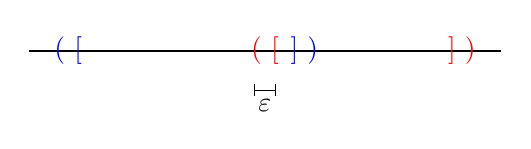
\begin{tikzpicture}
		\draw[thick] (0,0) -- (6,0);
		\node[blue] at (0.5,0) {$(\ [$};
		\node[blue] at (3.5,0) {$]\ )$};
		\node[red] at (3,0) {$(\ [$};
		\node[red] at (5.5,0) {$]\ )$};
		\draw[|-|] (2.86,-0.5) to node[midway, below] {$\varepsilon$} (3.135,-0.5);
	\end{tikzpicture}
%	\includegraphics[width=.5\textwidth]{open-to-closed-intervals}
	\caption{Replacing open intervals with closed intervals}
	\label{fig:open to closed interval}
\end{figure}

Finally, we order the endpoints of these intervals as $0 = s_0 < s_1 < s_2 < \cdots < s_n < s_{n + 1} = 1$. At each step, we made our intervals smaller, so each $[s_i, s_{i + 1}]$ is contained in some $S_{\alpha_i}$, hence $\gamma|_{[s_i, s_{i + 1}]}$ is a path in $A_{\alpha_i}$ by definition of $S_{\alpha_i}$. Define
\[
\gamma_i : I \xrightarrow{\text{linear squash}} [s_i, s_{i + 1}] \overset{\gamma}{\longrightarrow} A_{\alpha_i},
\]
and note that $\gamma_i(1) = \gamma(s_{i + 1}) = \gamma_{i + 1}(0)$ for all $i$. Now, by a reparametrization,
\[
\gamma \simeq \gamma_0 * \gamma_1 * \cdots * \gamma_n.
\]

Since each $A_{\alpha_i} \cap A_{\alpha_{i + 1}}$ is path-connected, let $p_i : I \to A_{\alpha_i} \cap A_{\alpha_{i + 1}}$ be a path from $x_0$ to $\gamma_i(1) = \gamma_{i + 1}(0)$. Then we can insert these paths along with their inverses in our expression for $\gamma$ without changing anything, since composing a path with its inverse is equivalent to doing nothing, up to path-homotopy. That is,
\[
\gamma \simeq \gamma_0 * \bar p_0 * p_0 * \gamma_1 * \bar p_1 * p_1 * \cdots * p_{n - 1} * \gamma_n.
\]
We think of traveling along $\gamma_0$, then to $x_0$ and back along $p_0$ and its inverse, then continuing along $\gamma_1$, and so on until we get all the way to $\gamma_n$, which takes us back to $x_0$.

\begin{figure}[h]
	\centering
	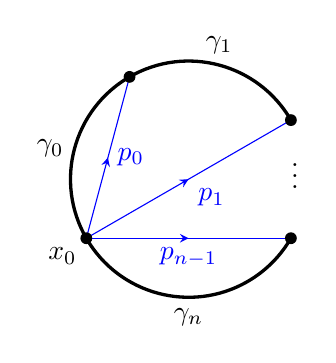
\begin{tikzpicture}[scale=1.5]
		\draw[blue, mid arrow] (210:1) to node[midway, below] {$p_{n - 1}$} (330:1);
		\draw[blue, mid arrow] (210:1) to node[midway, right] {$p_0$} (120:1);
		\draw[blue, mid arrow] (210:1) to node[midway, below right] {$p_1$} (30:1);
		\draw[very thick] (30:1) arc (30:120:1) node[midway, above] {$\gamma_1$} arc (120:210:1) node[midway, left] {$\gamma_0$} arc (210:330:1) node[midway, below] {$\gamma_n$};
		\node at (0.9,0.1) {$\vdots$};
		\foreach \t in {30, 120, 210, 330} {
			\fill (\t:1) circle (0.075/1.5);
		}
		\node[below left] at (210:1) {$x_0$};
	\end{tikzpicture}
	\caption{Final decomposition of $\gamma$}
	\label{fig:final loop decomp}
\end{figure}

Note that by construction, each $p_i * \gamma_{i + 1} * \bar p_{i + 1}$ is a loop in $A_{\alpha_{i + 1}}$ at $x_0$, so we have achieved our desired decomposition of $\gamma$. This tells us that we can use the elements of all the $\pi_1(A_\alpha, x_0)$ as generators for $\pi_1(X, x_0)$. To understand the relations, we will take a quick trip to the land of group theory.

\subsubsection{Free Products and Amalgamation}
Motivated by the free group on a set, we want to figure out a ``free'' way to combine groups that allows elements of different groups to interact with each other. The direct product is therefore not sufficient, since it doesn't allow interaction between elements of different groups. Instead, we will construct a free group, but be careful not to forget the group structure we started with in the original groups.

This will be helpful because it's exactly what we want to do with $\pi_1(A_\alpha, x_0)$. We want to combine the different groups to use as generators for $\pi_1(X, x_0)$, but we don't want to forget the original group structure we had in $A_\alpha$, since path composition/homotopy in $A_\alpha$ still works if you view it as living in $X$.

\begin{defi}
	Given two groups $G_1, G_2$, we define the \emph{free product} of $G_1$ and $G_2$ as
	\[
	G_1 * G_2 = \{\text{words in } G_1 \sqcup G_2 \text{, but we allow multiplication in } G_i\}
	\]
\end{defi}

More formally, $G_1 * G_2$ is the set of words in the alphabet $G_1 \sqcup G_2$, with relations that say for all $g, h \in G_i$,
\[
\underbrace{gh}_{\text{word with two letters}} = \underbrace{g \cdot h}_{\text{word with one letter}}
\]
where $g \cdot h$ is the single element of $G_i$ which is the product of $g$ and $h$. Also, we identify $e_1 = e_2$, where $e_i$ is the identity element of $G_i$. Note that this automatically identifies $e_i$ with the empty word, since if $w$ is any word then, then
\[
we_1 = we_2 = e_1w = e_2w = w
\]
because one of $e_1$ and $e_2$ must be in the same group as the last letter of $w$ and one of $e_1$ and $e_2$ must be in the same group as the first letter of $w$, so we can just let the multiplication happen within that group by the first kind of relation.

This also obviates the need for formal inverses, since the formal inverse of $g$ would be immediately identified with the actual inverse of $g$ in whatever group $g$ lives in (since $gg^{-1} = e = \text{``\ ''}$).

Most formally, we can write $G_1 * G_2$ with the presentation
\[
G_1 * G_2 = \left\langle G_1 \sqcup G_2 \ \middle|\ \begin{aligned}(g)(g') &= (gg')\quad \forall g, g' \in G_i,\\(e_1) &= (e_2)\end{aligned} \right\rangle,
\]
or, if $G_1 = \langle S_1 \mid R_1 \rangle$ and $G_2 = \langle S_2 \mid R_2 \rangle$, then
\[
G_1 * G_2 = \langle S_1 \sqcup S_2 \mid R_1 \sqcup R_2 \rangle.
\]

Abstractly, $G_1 * G_2$ is the coproduct of $G_1$ and $G_2$ in the category of groups. If you know what this means, write out the universal property and prove that it is satisfied by $G_1 * G_2$.
\bigskip

What if there is more structure on the groups that we don't want to forget? In particular, what if $G_1$ and $G_2$ share a common subgroup $H$? Under our definition of $G_1 * G_2$, there would be two copies of $H$. This doesn't seem quite right, since we should be able to multiply an element of $G_1$ by an element of $G_2$ if they are both in $H$.

In this case, it is actually somewhat more clear to use the abstract perspective to say that a common subgroup $H$ of $G_1$ and $G_2$ is really a pair of inclusion maps $i_1 : H \hookrightarrow G_1$ and $i_2 : H \hookrightarrow G_2$.

\begin{defi}
	The \emph{free product with amalgamation} of $G_1$ and $G_2$ with respect to $i_1$ and $i_2$ is $G_1 *_H G_2$, which is by definition $G_1 * G_2$ with the additional relations $i_1(h) = i_2(h)$ for all $h \in H$. This group has the presentation
	\[
	G_1 *_H G_2 = \left\langle G_1 \sqcup G_2 \ \middle|\ \begin{aligned}(g)(g') &= (gg')\quad \forall g, g' \in G_i,\\i_1(h) &= i_2(h)\quad \forall h \in H\end{aligned} \right\rangle,
	\]
	where we can reformulate the top relations in terms of generators if it is more convenient.
\end{defi}

Finally, note that we can generalize these definitions to take the free product of arbitrarily many groups and amalgamate over arbitrarily many common subgroups. In particular, if $\{G_\alpha\}_\alpha$ is a family of groups, then their free product is
\[
\bigast_\alpha G_\alpha = \left\langle \sqcup_\alpha G_\alpha \ \middle|\ \begin{aligned}(g)(g') &= (gg')\quad \forall g, g' \in G_\alpha,\\(e_\alpha) &= (e_\beta)\quad \forall \alpha, \beta\end{aligned} \right\rangle
\]

If we have some common subgroups $H_\beta$, where $H_\beta$ is common to a subfamily $\mathcal{G}_\beta \subseteq \{G_\alpha\}_\alpha$ (meaning that for all $G_\alpha \in \mathcal{G}_\beta$, there is an inclusion map $i_\beta^\alpha : H_\beta \hookrightarrow G_\alpha$), we define
\[
\bigast_\alpha\!_{i_\beta^\alpha}\ G_\alpha = \left\langle \bigsqcup_\alpha G_\alpha \ \middle|\ \begin{aligned}(g)(g') &= (gg')\quad \forall g, g' \in G_\alpha,\\i_\beta^\alpha(h) &= i_\beta^{\alpha'}(h)\quad \forall h \in H_\beta,\ \forall \alpha,\alpha'\end{aligned} \right\rangle
\]
Interpreting the second relation, it says that for all $h \in H_\beta$, all the images of $h$ in different $G_\alpha$'s are identified.

Of course, these presentations can be reformulated in terms of generators and relations for each $G_\alpha$ and $H_\beta$ when that is more convenient.

\begin{exer}
	Convince yourself that this general definition makes sense, or decide that you don't care and only want to think about the case of two groups (you will not lose too much in adopting the second approach).
\end{exer}

\subsubsection{Presenting $\pi_1$}
Let's go back to our goal of understanding the fundamental group by breaking down loops into loops in simpler subspaces. Recall that in our setting, we have a space $X$, a basepoint $x_0 \in X$, and a family of open, path-connected sets $\{A_\alpha\}_\alpha$ that cover $X$ such that $A_\alpha \cap A_\beta$ is also always path-connected. We can define a map 
\begin{align*}
	\bigast_\alpha \pi_1(A_\alpha, x_0) &\to \pi_1(X, x_0)\\
	[\gamma_1] [\gamma_2] \cdots [\gamma_n] &\mapsto [\gamma_1 * \gamma_2 * \cdots * \gamma_n],
\end{align*}
where we do path composition on $\gamma_1, \gamma_2, \ldots, \gamma_n$ by viewing them as loops in $X$ rather than loops in some $A_\alpha$. Our work in \cref{subsec:breaking loops} tells us that this map is actually surjective. The Seifert-van Kampen theorem gives us a stronger result if we additionally require the triple intersections $A_\alpha \cap A_\beta \cap A_\gamma$ to be path connected. Specifically, it tells us that we can make our map injective by amalgamating over all $\pi_1(A_\alpha \cap A_\beta, x_0)$ in the domain using the natural inclusion maps $i_{\alpha, \beta}^\alpha : \pi_1(A_\alpha \cap A_\beta, x_0) \hookrightarrow \pi_1(A_\alpha, x_0)$ given by $[\gamma] \mapsto [\gamma]$. Here we take a loop in $A_\alpha \cap A_\beta$ and view it instead a a loop in $A_\alpha$.

\begin{thm}[Seifert-van Kampen]
	If a space $X$ has a basepoint $x_0$ and is covered by some path-connected open sets $\{A_\alpha\}$ such that all double and triple intersections $A_\alpha \cap A_\beta$ and $A_\alpha \cap A_\beta \cap A_\gamma$ are path-connected and $x_0 \in A_\alpha$ for all $\alpha$, then
	\[
	\bigast_\alpha\!_{i_{\alpha, \beta}^\alpha} \pi_1(A_\alpha, x_0) \cong \pi_1(X, x_0)
	\]
	where $i_{\alpha, \beta}^\alpha : \pi_1(A_\alpha \cap A_\beta, x_0) \hookrightarrow \pi_1(A_\alpha, x_0)$ is the natural inclusion. Moreover, this isomorphism is given explicitly by the map $[\gamma_1] [\gamma_2] \cdots [\gamma_n] \mapsto [\gamma_1 * \gamma_2 * \cdots * \gamma_n]$.
\end{thm}

We will almost always be interested in the case where there are only two open sets $A$ and $B$, and in this case the condition that triple intersections are path-connected is vacuous.

\begin{thm}[Simplified Seifert-van Kampen]\label{thm:simplified van Kampen}
	If $X = A \cup B$ where $A$ and $B$ are open and path-connected, and $A \cap B$ contains $x_0$ and is path-connected, then
	\[
	\pi_1(X, x_0) = \pi_1(A, x_0) *_{\pi_1(A \cap B, x_0)} \pi_1(B, x_0).
	\]
\end{thm}

\begin{proof}
	We've already showed that the map is surjective. To prove that it's a group homomorphism, we check that the relations from the free group with amalgamation are safely carried into $\pi_1(X, x_0)$. First, if $[\gamma_1], [\gamma_2] \in \pi_1(A_\alpha, x_0)$, then
	\[
	[\gamma_1][\gamma_2] \mapsto [\gamma_1 * \gamma_2] \qquad\text{and}\qquad [\gamma_1 * \gamma_2] \mapsto [\gamma_1 * \gamma_2].
	\]
	Hence the free product relations are satisfied. If $[\gamma] \in \pi_1(A_\alpha \cap A_\beta, x_0)$, then denoting the images of $[\gamma]$ in $\pi_1(A_\alpha, x_0)$ and $\pi_1(A_\beta, x_0)$ by $[\gamma]_\alpha$ and $[\gamma]_\beta$, respectively, we have
	\[
	[\gamma]_\alpha \mapsto [\gamma] \qquad\text{and}\qquad [\gamma]_\beta] \mapsto [\gamma],
	\]
	so the amalgamation relations are also satisfied. Finally, we need to show injectivity. That is, we need to show that if
	\[
	[\gamma_1 * \gamma_2 * \cdots * \gamma_n] = [\delta_1 * \delta_2 * \cdots * \delta_m],
	\]
	where $\gamma_i \in \pi_1(A_{\alpha_i}, x_0)$ and $\delta_j \in \pi_1(A_{\alpha_j}, x_0)$, then the path composition of the $\gamma_i$'s and the path composition of the $\delta_j$'s are related (up to homotopy) by a sequence of free product and amalgamation relations (so that the corresponding words, which are the preimages, are the same element in the free product with amalgamation). The details of this are very technical; essentially, if we denote $\gamma = \gamma_1 * \gamma_2 * \cdots * \gamma_n$ and $\delta = \delta_1 * \delta_2 * \cdots * \delta_m$, then we have a path-homotopy $H : I \times I \to X$ showing $\gamma \simeq \delta$. By breaking up the square $I \times I$, we can get the sequence of relations that we want. Those interested in more details can find them in Hatcher's \cite{H} proof in Section 1.2, available online (legally) for free.
\end{proof}

\subsection{Homotopy Equivalence}\label{sec:homotopy}
Our other main idea for computing fundamental groups will be deforming spaces in ways that don't affect the fundamental group. Homeomorphisms already provide some ways to deform spaces, but they're still stricter than we need to be, since for instance it seems like an open annulus should have the same fundamental group as $S^1$, and that our technique for $S^1$ should also apply to the annulus, but this is not entirely clear since for instance you can have nonconstant trivial loops in the annulus but not in $S^1$. However, it turns out that $S^1$ and the annulus are homotopy equivalent even though they're not homeomorphic, so they must have isomorphic fundamental groups.

\subsubsection{Homotopy with Maps and Spaces}
To define a homotopy equivalence, we first need to define a homotopy. Homotopies generalize the path-homotopies we worked with to define the fundamental group to work with arbitrary continuous maps, not just paths.

\begin{defi}
	Let $f, g : X \to Y$ be maps. A \emph{homotopy} from $f$ to $g$ is a map $H : I \times X \to Y$, written $H(t, x) = H_t(x)$, such that $H_0 = f$ and $H_1 = g$. When there is a homotopy $H$ from $f$ to $g$, we write $f \simeq g$ via $H$.
\end{defi}

Just as we can think of path-homotopies as paths in the space of paths, we can think of homotopies as paths in the space of functions $X \to Y$. Equivalently, a homotopy is a fmaily of continuous maps $X \to Y$ that continuously interpolates between $f$ and $g$.

\begin{exa}
	All path-homotopies are homotopies. However, there are homotopies of paths that are not path-homotopies, since homotopies don't require the endpoints to be fixed. See, for example, \cref{fig:non-path homotopy}.
	
	\begin{figure}[h]
		\centering
		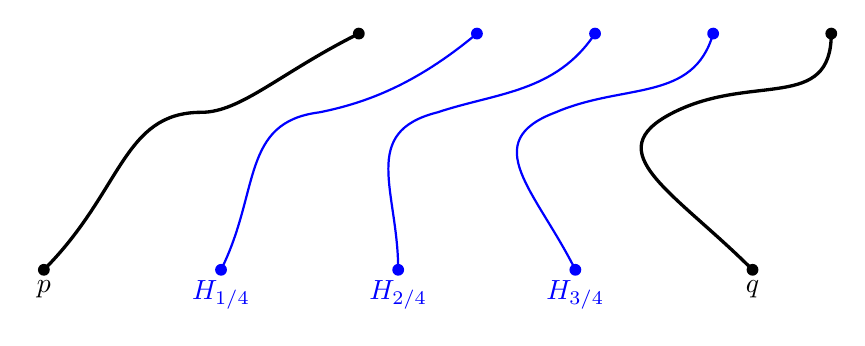
\begin{tikzpicture}
			\draw[very thick]
				(0,0) .. controls +(1,1) and +(-1,0) .. node[pos=0, below] {$p$}
				(2,2) .. controls +(0.5,0) and +(-1,-0.5) .. (4,3);
				\fill (0,0) circle (0.075);
				\fill (4,3) circle (0.075);
			\foreach \t in {1,2,3} {
				\begin{scope}[shift={(2*\t,0)}]
					\draw[thick, blue]
						(0 + \t/4,0) .. controls +(1 - \t/2,1) and +(-1,0 - \t/8) .. node[pos=0, below] {$H_{\t/4}$}
						(2 - \t/2,2) .. controls +(0.5 + \t/8,0 + \t/8) and +(-1 + \t/4,-0.5 - \t/8) .. (4 - \t/2,3);
						\fill[blue] (0 + \t/4,0) circle (0.075);
						\fill[blue] (4 - \t/2,3) circle (0.075);
				\end{scope}
			}
			\begin{scope}[shift={(8,0)}]
				\draw[very thick]
					(1,0) .. controls +(-1,1) and +(-1,-0.5) .. node[pos=0, below] {$q$}
					(0,2) .. controls +(1,0.5) and +(0,-1) .. (2,3);
				\fill (1,0) circle (0.075);
				\fill (2,3) circle (0.075);
			\end{scope}
		\end{tikzpicture}
		\caption{A homotopy of paths which is not a path-homotopy}
		\label{fig:non-path homotopy}
	\end{figure}
	
	Note that without requiring the endpoints of a path to be fixed, all paths are basically boring, in that every path is homotopic to a constant map. Formally, if $p : I \to X$ is a path, then the homotopy $H_t$ given by $H_t(s) = p(s - ts)$ starts with $p$ and ends with the constant path at $p(0)$. This can be seen visually in \cref{fig:paths are boring}.
	
	\begin{figure}[h]
		\centering
		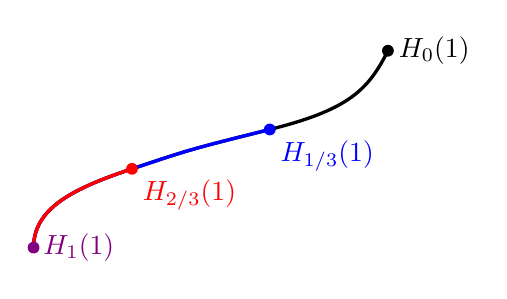
\begin{tikzpicture}
			\draw[very thick]
				(0,0) .. controls +(0,0.5) and +(-0.75,-0.25) ..
				(1.25,1) .. controls +(0.75,0.25) and +(-1,-0.25) ..
				(3,1.5) .. controls +(1,0.25) and +(-0.25, -0.5) .. (4.5,2.5) node[pos=1, right] {$H_0(1)$};
			\fill (4.5,2.5) circle (0.075);
			\draw[very thick, blue]
				(0,0) .. controls +(0,0.5) and +(-0.75,-0.25) ..
				(1.25,1) .. controls +(0.75,0.25) and +(-1,-0.25) ..
				(3,1.5) node[pos=1, below right] {$H_{1/3}(1)$};
			\fill[blue] (3,1.5) circle (0.075);
			\draw[very thick, red]
				(0,0) .. controls +(0,0.5) and +(-0.75,-0.25) ..
				(1.25,1) node[pos=1, below right] {$H_{2/3}(1)$};
			\fill[red] (1.25,1) circle (0.075);
			\fill[violet] (0,0)  circle (0.075);
			\node[violet, right] {$H_1(1)$};
		\end{tikzpicture}
		\caption{Homotopy from a path to the constant path}
		\label{fig:paths are boring}
	\end{figure}
\end{exa}

\begin{exa}
	A path is a homotopy between constant maps.
\end{exa}

\begin{exa}
	In $\R^n$, we can again use the straight-line homotopy to get a homotopy betweeen any two maps. Formally, if $f, g : X \to \R^n$, define $H : I \times X \to \R^n$ by
	\[
	H_t(x) = tg(x) + (1 - t)f(x).
	\]
	Then $H$ is continuous and $H_0 = f$, $H_1 = g$, so $f \simeq g$. As with path-homotopies, this actually works for any maps to a convex subset of $\R^n$.
\end{exa}

\begin{exa}
	Every path is homotopic to a constant map. We show this by applying the straight-line homotopy to $I$: given $p : I \to Y$, define $H : I \times I \to Y$ by $H_t(s) = p(s - ts)$. Then $H_0 = p$ while $H_1$ is the constant map at $p(0)$. This is why the condition that path-homotopies fix the endpoints throughout is crucial. In fact, what we are doing here is reparametrizing $p$ with a map $I \to I$ that doesn't fix $0$ and $1$, which is not permissible for path-homotopies but is perfectly fine for homotopies.
\end{exa}

\begin{exer}
	What is a good analogy for reparametrizations in the setting of homotopies rather than path-homotopies? Prove that a reparametrization is homotopic to the original map.
\end{exer}

\begin{prop}
	Homotopy is an equivalence relation.
\end{prop}

\begin{proof}
	The proof is identical to the proof for path-homotopies, except we don't need to check anything like the endpoints being fixed by all maps so the proof here is even shorter.
\end{proof}

An equivalence class of maps under $\simeq$ is called a \emph{homotopy class}. It's also a good idea to check that homotopy plays nicely with composition (now we are actually talking about function composition, not composition of paths).

\begin{lem}\label{lem:homotopy composition}
	If $f, f' : X \to Y$ are homotopic via $F$ and $g : Y \to Z$, then $g \circ f \simeq g \circ f'$ via the homotopy $H_t = g \circ F_t$. If $f : X \to Y$ and $g, g' : Y \to Z$ are homotopic via $G$, then $g \circ f \simeq g' \circ f$ via the homotopy $H'_t = G_t \circ f$.\qed
\end{lem}

\begin{cor}
	If $f, f' : X \to Y$ are homotopic and $g, g' : Y \to Z$ are homotopic, then $g \circ f \simeq g' \circ f'$.
\end{cor}

\begin{proof}
	By \cref{lem:homotopy composition}, $f \circ g \simeq f \circ g' \simeq f' \circ g'$, hence $f \circ g \simeq f' \circ g'$.
\end{proof}

For those familiar with abstract nonsense, this implies that topological spaces with homotopy classes of maps form a category.

We now want to use our new notion of equivalence of maps to define a way to think about equivalence of spaces. In particular, hopefully this new equivalence will allow us to deform spaces in more ways, but still preserve the fundamental group. Recall that two spaces $X, Y$ are homeomorphic if there are maps $f : X \to Y$ and $g : Y \to X$ such that $g \circ f = \mathrm{id}_X$ and $f \circ g = \mathrm{id}_Y$. The rigidity in this definition comes from the fact that $g \circ f$ and $f \circ g$ must be literally equal to the identity, so to give ourselves some more wiggle room, we will allow these maps to be only homotopic to the identity.

\begin{defi}
	Two spaces $X, Y$ are \emph{homotopy equivalent} if there are maps $f : X \to Y$ and $g : Y \to X$ such that $g \circ f \simeq \mathrm{id}_X$ and $f \circ g \simeq \mathrm{id}_Y$. These maps $f, g$ are called \emph{homotopy inverses}, and if they exist then we write $X \simeq Y$ and say $X$ and $Y$ have the same \emph{homotopy type}.
\end{defi}

As we will prove shortly, homotopy equivalence is a fine way to think about spaces being equivalent, but it is strictly weaker than homeomorphism. One way to think about homotopy equivalence is that the condition $g \circ f \simeq \mathrm{id}_X$ means there is a way to choose a path from each point in $X$ to its image under $f \circ g$. So a homotopy equivalence is a way to push the points in a space around in a continuous way.

\begin{exa}
	$\R^n$ has the homotopy type of a point. If $\{a\}$ is a point (meaning a space with one element), then there is only one map $f : \R^n \to \{a\}$. With any  map $g : \{a\} \to \R^n$, we have $g \circ f = \mathrm{id}_{\R^n}$ because any pair of maps to $\R^n$ are homotopic and $f \circ g = \mathrm{\{a\}}_*$ because there is only one map $\{a\} \to \{a\}$. Thus, homotopy type is not enough to distinguish between $\R^n$ and $\R^m$ since they both hace the homotopy type of a point. In particular, homotopy equivalence doesn't preserve dimension.
\end{exa}

We will see more examples of homotopy equivalences in \cref{sec:examples}. We should prove that homotopy equivalence is actually a reasonable notion of equivalence.

\begin{prop}
	Homotopy equivalence is an equivalence relation.
\end{prop}

\begin{proof}
	For any space $X$, $\mathrm{id}_X : X \to X$ is a homotopy equivalence. If $X \simeq Y$ with $f : X \to Y$ and $g : Y \to X$ homotopy inverses, then $g : Y \to X$ is a homotopy equivalence showing $Y \simeq X$. Finally, if $a : X \to Y$ and $b : Y \to X$ are homotopy inverses and $c : Y \to Z$ and $d : Z \to Y$ are homotopy inverses, then
	\[
	(c \circ a) \circ (b \circ d) = c \circ (a \circ b) \circ d \simeq c \circ \mathrm{id}_Y \circ d = c \circ d \simeq \mathrm{id}_Z
	\]
	and
	\[
	(b \circ d) \circ (c \circ a) = b \circ (d \circ c) \circ a \simeq b \circ \mathrm{id}_Y \circ a = b \circ a \simeq \mathrm{id}_X
	\]
	Thus $c \circ a : X \to Z$ and $b \circ d : Z \to X$ are homotopy inverses, so $X \simeq Z$.
\end{proof}

From this proposition, we should get some kind of statement about a category of homotopy equivalence classes of spaces with homotopy classes of maps. If you enjoy abstract nonsense, make this definition precise.
\bigskip

One detail to bring up is the notion of \emph{pointed} spaces and maps. Recall that when we defined path-homotopies, we wanted the endpoints of the paths to be fixed throughout all time because the endpoints are an important part of the ``structure'' of a path. When talking about the fundamental group, an important part of the structure is the basepoint, since we know that changing base point can completely change the fundamental group. So, we don't really want our homotopies to move the base points around while deforming a map.

In order to resolve this concern, we will consider spaces with a fixed basepoint, so a special point is part of the data of the structure we are looking at. That is, we will now consider pairs $(X, x_0)$ where $X$ is a space and $x_0 \in X$ is a fixed point, which are called \emph{pointed spaces}. A \emph{pointed map} $f : (X, x_0) \to (Y, y_0)$ is a map $X \to Y$ which takes $x_0$ to $y_0$. If $f, g : (X, x_0) \to (Y, y_0)$ are two pointed maps, then a \emph{pointed homotopy} from $f$ to $g$ is a map $H : I \times X \to Y$ such that $H_t : (X, x_0) \to (Y, y_0)$ is a pointed map for all $t \in I$ and such that $H_0 = f$, $H_1 = g$. That is, a pointed homotopy from $f$ to $g$ is a homotopy from $f$ to $g$ in which all the intermediate maps are also pointed.

Pointed homotopies satisfy all the properties we just proved for homotopies, including defining pointed homotopy equivalences. The pointed condition makes the statements we will prove easier to state and prove, but not much is lost by ignoring it almost all the time when reading the statements and proofs.

\medskip
\noindent\textbf{For the remainder of this section, all homotopies and homotopy equivalences are assumed to be pointed.}

\subsubsection{Homotopy Invariance of the Fundamental Group}
In order to use homotopy equivalence as a tool for computing the fundamental group (or at least showing that the fundamental groups of two spaces must be isomorphic), we need to show that homotopy equivalences induce isomorphisms on the fundamental group.

\begin{defi}
	Given a map $f : (X, x_0) \to (Y, y_0)$, the \emph{induced map} $f_* : \pi_1(X, x_0) \to \pi_1(Y, y_0)$ is given by $f_*([\gamma]) = [f \circ \gamma]$.
\end{defi}

The important properties of the induced map are the following.

\begin{prop}
	Let $f : (X, x_0) \to (Y, y_0)$ be a map and $f_* : \pi_1(X, x_0) \to \pi_1(Y, y_0)$ be the induced map on fundamental groups. Then
	\begin{enumerate}
		\item $f_*$ is well-defined on path-homotopy classes.
		\item $f_*$ is a group homomorphism.
		\item If $f : (X, x_0) \to (Y, y_0)$ and $g : (Y, y_0) \to (Z, z_0)$, then $(g \circ f)_* = g_* \circ f_*$.
		\item $(\mathrm{id}_X)_* = \mathrm{id}_{\pi_1(X, x_0)}$.
	\end{enumerate}
\end{prop}

\begin{proof}
	For \emph{1}, if $\gamma \simeq \gamma'$ are path-homotopic via $H_t$, then $f \circ \gamma$ and $f \circ \gamma'$ are path-homotopic via $f \circ H_t$.
	
	For $\emph{2}$, it suffices to note that $f \circ (\alpha * \beta) = (f \circ \alpha) * (f \circ \beta)$, which follows from writing out the definition of composition of paths:
	\[
	f \circ (\alpha * \beta)(s) = f\left(\begin{cases}
		\alpha(s) & \text{if } s \leq 1/2\\
		\beta(s) & \text{if } s \geq 1/2
	\end{cases}\right) = \begin{cases}
		f \circ \alpha(s) & \text{if } s \leq 1/2\\
		f \circ \beta(s) & \text{if } s \geq 1/2
	\end{cases} = (f \circ \alpha) * (f \circ \beta)(s).
	\]
	
	For \emph{3}, for all $[\gamma] \in \pi_1(X, x_0)$ we have
	\[
	(g \circ f)_*([\gamma]) = [g \circ f \circ \gamma] = g_*([f \circ \gamma]) = (g_* \circ f_*)([\gamma]).
	\]
	
	Finally, for \emph{4}, for all $[\gamma] \in \pi_1(X, x_0)$ we have $[\mathrm{id}_X \circ \gamma] = [\gamma]$, hence $(\mathrm{id}_X)_* = \mathrm{id}_{\pi_1(X, x_0)}$.
\end{proof}

In the language of abstract nonsense, we have just proved that $\pi_1$ is a functor from pointed topological spaces to groups.

As we originally noted, we want to show that homotopy equivalences induce isomorphisms on the fundamental group. Now we can say more precisely that we want to show that if $f : X \to Y$ is a homotopy equivalence, then $f_*$ is an isomorphism. To show this, it suffices to show that homotopic maps induce the same map on fundamental groups, since then if $f : X \to Y$ is a homotopy equivalence with homotopy inverse $g : Y \to X$, $(g \circ f)_* = g_* \circ f_*$ and $(f \circ g)_* = f_* \circ g_*$ are the identity group homomorphisms because $g \circ f$ and $f \circ g$ are homotopic to the identities.

\begin{prop}
	If $f, g : (X, x_0) \to (Y, y_0)$ are homotopic, then $f_* = g_*$.
\end{prop}

\begin{proof}
	Let $H_t$ be a homotopy from $f$ to $g$. Then since each $H_t$ takes $x_0$ to $y_0$ (by definition of a pointed homotopy), for all loops $\gamma$ at $x_0$, $f \circ \gamma \simeq g \circ \gamma$ (path-homotopy) via $H_t \circ \gamma$. Hence $[f \circ \gamma] = [g \circ \gamma]$, proving that $f_* = g_*$.
\end{proof}

\begin{cor}\label{cor:homotopy invariance}
	If $f : (X, x_0) \to (Y, y_0)$ is a homotopy equivalence, then $f_* :\pi_1(X, x_0) \to \pi_1(Y, y_0)$ is an isomorphism.
\end{cor}

\begin{proof}
	By definition, there exists a $g : (Y, y_0) \to (X, x_0)$ such that $g \circ f \simeq \mathrm{id}_X$ and $f \circ g \simeq \mathrm{id}_Y$. Hence $g_* \circ f_* = \mathrm{id}_{\pi_1(X, x_0)}$ and $f_* \circ g_* = \mathrm{id}_{\pi_1(Y, y_0)}$, so $f_*$ is an isomorphism.
\end{proof}

\subsection{Concrete Examples}\label{sec:examples}
Now that we have all these theoretical tools, let's use them to compute the fundamental group of some familiar spaces!

\begin{exa}\label{exa:compute annulus}
	Consider the open annulus $A$, which formally is an open disk minus a smaller open disk. Note that the basepoint we choose doesn't matter, since $A$ is path-connected. Then $A \simeq S^1$ via the homotopy that pulls each point in toward the centerline of the annulus, as shown in \cref{fig:annulus}.
	
	\begin{figure}[h]
		\centering
		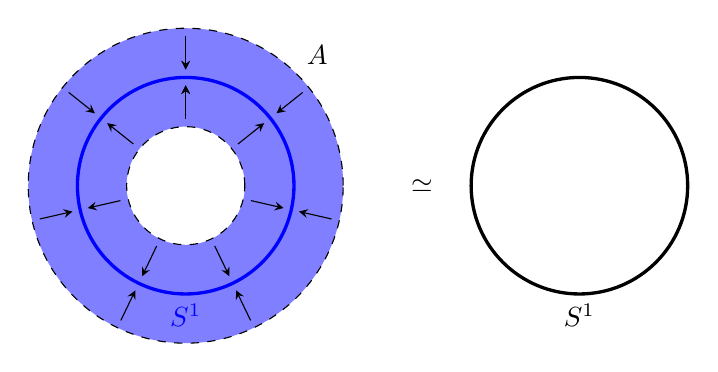
\begin{tikzpicture}
			\fill[opacity=0.5, blue] (0,0) circle (2);
			\fill[white] (0,0) circle (0.75);
			\draw[dashed] (0,0) circle (0.75);
			\draw[dashed] (0,0) circle (2);
			\draw[very thick, blue] (0,0) circle (1.375);
			\node[below, blue] at (0,-1.375) {$S^1$};
			\node[above right] at (1.41421356237,1.41421356237) {$A$};
			\begin{scope}[rotate=90]
			\foreach \t in {0,...,7} {
				\draw[-stealth] (\t*360/7:2 - 0.1) -- (\t*360/7:1.375 + 0.1);
				\draw[-stealth] (\t*360/7:0.75 + 0.1) -- (\t*360/7:1.375 - 0.1);
			}
			\end{scope}
			
			\node at (3,0) {$\simeq$};
			
			\draw[very thick] (5,0) circle (1.375);
			\node[below] at (5,-1.375) {$S^1$};
		\end{tikzpicture}
		\caption{The annulus is homotopy equivalent to $S^1$}
		\label{fig:annulus}
	\end{figure}
	
	Hence the inclusion $S^1 \hookrightarrow A$ is a homotopy equivalence, so $\pi_1(A, x_0) \cong \Z$ and moreover $\pi_1(A, x_0)$ is generated by the (path-homotopy class of the) loop that goes around the annulus once, since this is the image of the loop that goes around the circle once.
\end{exa}

\begin{exa}\label{exa:compute annulus}
	Now, let's compute that fundamental group of the torus $T$. We will do this in two ways. First, note that one way to define the torus is as the product of $S^1$ with itself: $T = S^1 \times S^1$. To see this, you can imagine placing a copy of $S^1$ at each point along another copy of $S^1$, which exactly creates the surface of the torus. Now, from an exercise from the original notes on the fundamental group, we know the $\pi_1$ preserves products. Again, the basepoint we choose doesn't matter because $T$ is path connected, so we have
	\[
	\pi_1(T, x_0) = \pi_1(S^1 \times S^1, (x_1, x_2)) \cong \pi_1(S_1, x_1) \times \pi_1(S_1, x_2) \cong \Z \times \Z
	\]
	since we have already seen that $\pi_1(S^1, x_0) \cong \Z$. However, there's another way that will let us use our new tools. The torus can also be expressed as a quotient of the square by gluing opposite edges in the same direction, as shown in \cref{fig:torus from square}.
	
	\begin{figure}[h]
		\centering
		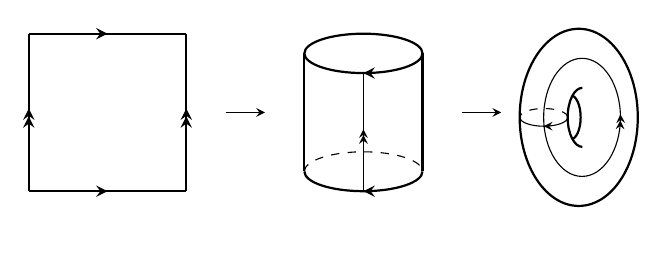
\begin{tikzpicture}
			\draw[thick, mid arrow,] (0,0) -- (2,0);
			\draw[thick, mid arrow] (0,2) -- (2,2);
			\draw[thick, double mid arrow] (0,0) -- (0,2);
			\draw[thick, double mid arrow] (2,0) -- (2,2);
			
			\draw[-stealth] (2.5,1) -- (3,1);
			
			\begin{scope}[shift={(4.5,0)}]
				\draw[thick] (-1,1.75) arc (180:0:0.75 and 0.25);
				\draw[thick, mid arrow] (0.5,1.75) arc (0:180:0.75 and -0.25);
				\draw[dashed] (-1,0.25) arc (180:0:0.75 and 0.25);
				\draw[thick, mid arrow] (0.5,0.25) arc (0:180:0.75 and -0.25);
				\draw[thick] (-1,0.25) -- (-1,1.75);
				\draw[thick] (0.5,0.25) -- (0.5,1.75);
				\draw[double mid arrow] (-0.25,0) -- (-0.25,1.5);
			\end{scope}
			
			\draw[-stealth] (5.5,1) -- (6,1);
			
			\begin{scope}[scale=0.75, shift={(9,1.25)}, rotate=-90]
				\draw[thick] (0,0.3125) ellipse (1.5 and 1);
				\begin{scope}
					\clip (-1,0) rectangle (2,0.375);
					\draw[thick] (0,0.375) ellipse (0.5 and 0.25);
				\end{scope}
				
				\begin{scope}
					\clip (0,0.375) ellipse (0.5 and 0.25);
					\draw[thick] (0,0.1725) ellipse (0.375 and 0.1725);
				\end{scope}
				
				\draw[mid arrow] (0,0.125) arc (90:-90:0.15 and 0.405);
				\draw[dashed] (0,0.125) arc (90:-90:-0.15 and 0.405);
				\draw[double mid arrow close] (0,-0.28125) arc (-90:270:1 and 0.65);
			\end{scope}
		\end{tikzpicture}
		\caption{The torus as a quotient of the square}
		\label{fig:torus from square}
	\end{figure}
	
	We can cover the square with two open sets $A$ and $B$, where $A$ is a neighborhood of the boundary and $B$ is a disk at the center of the circle (see \cref{fig:covering torus}). As long as we make these sets overlap and choose a basepoint in the intersection, by van Kampen's theorem we have
	\[
	\pi_1(T, x_0) = \pi_1(A, x_0) *_{\pi_1(A \cap B, x_0)} \pi_1(B, x_0).
	\]
	
	\begin{figure}[h]
		\centering
		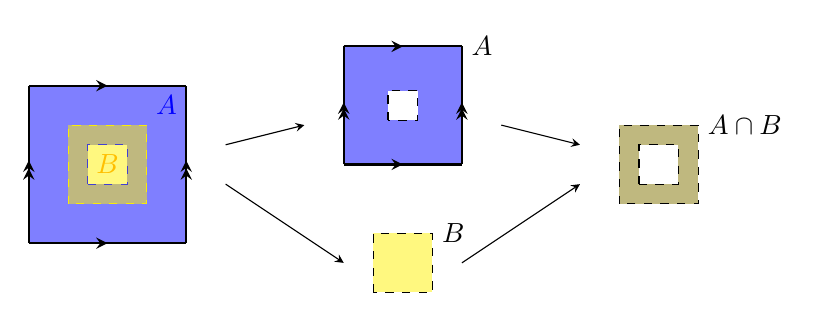
\begin{tikzpicture}
			\fill[blue, opacity=0.5] (0,0) rectangle (2,2);
			\fill[white] (0.75,0.75) rectangle (1.25,1.25);
			\fill[yellow, opacity=0.5] (0.5,0.5) rectangle (1.5,1.5);
			\node[blue] at (1.75,1.75) {$A$};
			\node[orange!50!yellow] at (1,1) {$B$};
			\draw[dashed, yellow, opacity=0.9] (0.5,0.5) rectangle (1.5,1.5);
			\draw[dashed, blue, opacity=0.65] (0.75,0.75) rectangle (1.25,1.25);
			\draw[thick, mid arrow,] (0,0) -- (2,0);
			\draw[thick, mid arrow] (0,2) -- (2,2);
			\draw[thick, double mid arrow] (0,0) -- (0,2);
			\draw[thick, double mid arrow] (2,0) -- (2,2);
			
			\draw[-stealth] (2.5,1.25) -- (3.5,1.5);
			\draw[-stealth] (2.5,0.75) -- (4,-0.25);
			
			\begin{scope}[shift={(4,1)}, scale=0.75]
				\fill[blue, opacity=0.5] (0,0) rectangle (2,2);
				\fill[white] (0.75,0.75) rectangle (1.25,1.25);
				\draw[dashed] (0.75,0.75) rectangle (1.25,1.25);
				\draw[thick, mid arrow,] (0,0) -- (2,0);
				\draw[thick, mid arrow] (0,2) -- (2,2);
				\draw[thick, double mid arrow] (0,0) -- (0,2);
				\draw[thick, double mid arrow] (2,0) -- (2,2);
				\node[right] at (2,2) {$A$};
			\end{scope}
			
			\begin{scope}[shift={(4,-1)}, scale=0.75]
				\fill[yellow, opacity=0.5] (0.5,0.5) rectangle (1.5,1.5);
				\draw[dashed] (0.5,0.5) rectangle (1.5,1.5);
				\node[right] at (1.5,1.5) {$B$};
			\end{scope}
			
			\draw[-stealth] (6,1.5) -- (7,1.25);
			\draw[-stealth] (5.5,-0.25) -- (7,0.75);
			
			\begin{scope}[shift={(7,0)}]
				\fill[blue, opacity=0.5] (0.5,0.5) rectangle (1.5,1.5);
				\fill[yellow, opacity=0.5] (0.5,0.5) rectangle (1.5,1.5);
				\fill[white] (0.75,0.75) rectangle (1.25,1.25);
				\draw[dashed] (0.5,0.5) rectangle (1.5,1.5);
				\draw[dashed] (0.75,0.75) rectangle (1.25,1.25);
				\node[right] at (1.5,1.5) {$A \cap B$};
			\end{scope}
		\end{tikzpicture}
		\caption{Covering the square (really, the torus) with open sets}
		\label{fig:covering torus}
	\end{figure}
	
	Therefore, we want to understand $\pi_1(A, x_0)$, $\pi_1(A \cap B, x_0)$, and $\pi_1(B, x_0)$. These are in opposite order of difficulty, so we will start with $\pi_1(B, x_0)$. Since $B$ is homeomorphic to a disk, which is a convex subset of $\R^2$, we know that $\pi_1(B, x_0)$ must be trivial (recall our computation using the straigh-line homotopy). Next, $\pi_1(A \cap B, x_0)$ is homeomorphic to the open annulus, so from \cref{exa:compute annulus} we know that $\pi_1(A \cap B, x_0) \cong \Z$, generated by a loop that goes around once.
	
	Now, we need to handle $A$. The first thing we need to do is use a homotopy equivalence to get $A$ into a more manageable form. We can push all the points out toward the boundary of the square, on to the lines that are being glued together. Then, after following the gluing instructions as in \cref{fig:homotope A}, we have a space $X$ consisting of two tangent circles. We will use van Kampen's theorem to compute the fundamental group of this space.
	
	\begin{figure}[h]
		\centering
		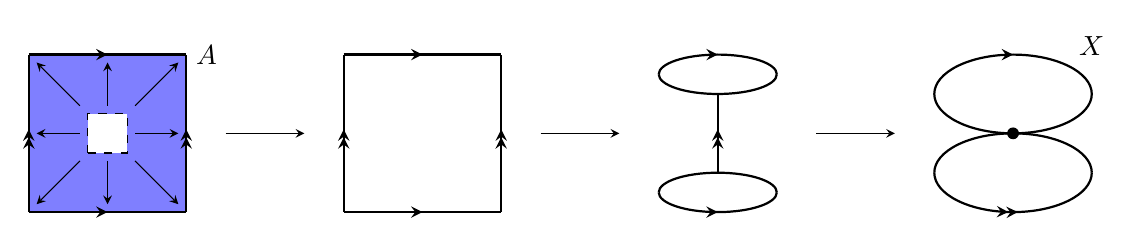
\begin{tikzpicture}
			\fill[blue, opacity=0.5] (0,0) rectangle (2,2);
			\fill[white] (0.75,0.75) rectangle (1.25,1.25);
			\draw[dashed] (0.75,0.75) rectangle (1.25,1.25);
			\draw[thick, mid arrow] (0,0) -- (2,0);
			\draw[thick, mid arrow] (0,2) -- (2,2);
			\draw[thick, double mid arrow] (0,0) -- (0,2);
			\draw[thick, double mid arrow] (2,0) -- (2,2);
			\node[right] at (2,2) {$A$};
			\draw[-stealth] (1.35,1) -- (1.9,1);
			\draw[-stealth] (1,1.35) -- (1,1.9);
			\draw[-stealth] (0.65,1) -- (0.1,1);
			\draw[-stealth] (1,0.65) -- (1,0.1);
			\draw[-stealth] (1.35,1.35) -- (1.9,1.9);
			\draw[-stealth] (0.65,1.35) -- (0.1,1.9);
			\draw[-stealth] (0.65,0.65) -- (0.1,0.1);
			\draw[-stealth] (1.35,0.65) -- (1.9,0.1);
			
			\draw[-stealth] (2.5,1) -- (3.5,1);
			
			\draw[thick, mid arrow] (4,0) -- (6,0);
			\draw[thick, mid arrow] (4,2) -- (6,2);
			\draw[thick, double mid arrow] (4,0) -- (4,2);
			\draw[thick, double mid arrow] (6,0) -- (6,2);
			
			\draw[-stealth] (6.5,1) -- (7.5,1);
			
			\begin{scope}[shift={(9,0)}]
				\draw[thick, mid arrow] (-1,1.75) arc (180:0:0.75 and 0.25);
				\draw[thick] (0.5,1.75) arc (0:180:0.75 and -0.25);
				\draw[thick] (-1,0.25) arc (180:0:0.75 and 0.25);
				\draw[thick, mid arrow] (-1,0.25) arc (180:0:0.75 and -0.25);
				\draw[thick, double mid arrow wide] (-0.25,0.5) -- (-0.25,1.5);
			\end{scope}
			
			\draw[-stealth] (10,1) -- (11,1);
			
			\draw[thick, mid arrow] (11.5,1.5) arc (180:0:1 and 0.5) node[above right, pos=0.75] {$X$};
			\draw[thick] (11.5,1.5) arc (180:0:1 and -0.5);
			\draw[thick] (11.5,0.5) arc (180:0:1 and 0.5);
			\draw[thick, double mid arrow] (11.5,0.5) arc (180:0:1 and -0.5);
			\fill (12.5,1) circle (0.075);
   		\end{tikzpicture}
		\caption{Simplifying $A$ using homotopy equivalence}
		\label{fig:homotope A}
	\end{figure}
	
	Note that the two circles themselves are not open subsets of $X$, but we can take small open neighborhoods of each circle to obtain open sets $U$ and $V$ that are each homotopy equivalent to $S^1$. Since $U$ and $V$ are open and path-connected and $U \cap V$ is path-connected and contains the tangent point, by van Kampen's theorem we have
	\[
	\pi_1(X, x_0) \cong \pi_1(U, x_0) *_{\pi_1(U \cap V, x_0)} \pi_1(V, x_0).
	\]
	But $U \cap V$ is homotopy equivalent to a point, since we can just shrink down all four ``arms'' of $U \cap V$ in toward the center. Hence $\pi_1(U \cap V, x_0)$ is trivial, so $\pi_1(X, x_0) \cong \Z * \Z$ because $U, V \simeq S^1$. In particular, $\pi_1(X, x_0)$ is generated by the two loops $\alpha, \beta$ that go around the circles in $X$, since these are the images of the generator of $\pi_1(S^1, x_0)$. Within $\pi_1(U, x_0)$ and $\pi_1(V, x_0)$, there are no relations on $\alpha$ or $\beta$ because $\Z$ is free on its generator. There are no relations induced by amalgamating over the trivial group, either, so in fact $\pi_1(X, x_0)$ is free on $\alpha$ and $\beta$.
	
	\begin{figure}[h]
		\centering
		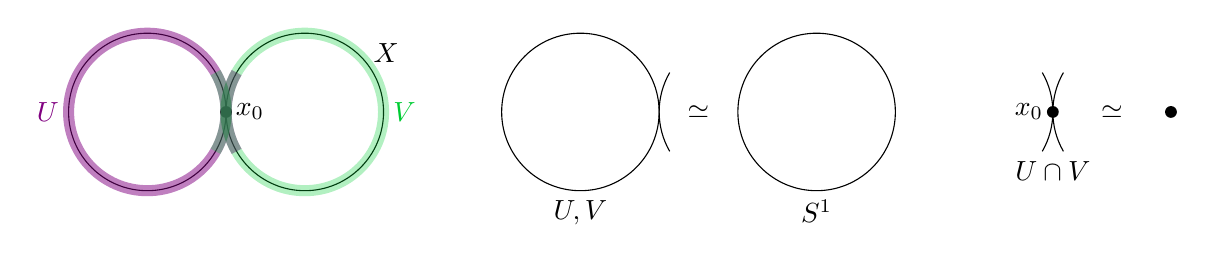
\begin{tikzpicture}
			\draw (0,0) circle (1);
			\draw (2,0) circle (1);
			\fill (1,0) circle (0.075);
			\node[right] at (1,0) {$x_0$};
			\node[above right] at (2.75,0.5) {$X$};
			\draw[line width=4, violet, opacity=0.5] (0,0) circle (1);
			\draw[line width=4, violet, opacity=0.5] (1,0) arc (180:150:1) arc (150:210:1);
			\node[left, violet] at (-1,0) {$U$};
			\draw[line width=4, green!80!blue, opacity=0.3] (2,0) circle (1);
			\draw[line width=4, green!80!blue, opacity=0.3] (1,0) arc (0:30:1) arc (30:-30:1);
			\node[right, green!80!blue] at (3,0) {$V$};
			
			\begin{scope}[shift={(5.5,0)}]
				\draw (0,0) circle (1);
				\draw (1,0) arc (180:150:1) arc (150:210:1);
				\node[below] at (0,-1) {$U, V$};
				\node at (1.5,0) {$\simeq$};
				\draw (3,0) circle (1);
				\node[below] at (3,-1) {$S^1$};
			\end{scope}
			
			\begin{scope}[shift={(11.5,0)}]
				\draw (0,0) arc (180:150:1) arc (150:210:1);
				\draw (0,0) arc (0:30:1) arc (30:-30:1);
				\fill (0,0) circle (0.075);
				\node[left] at (0,0) {$x_0$};
				\node[below] at (0,-0.5) {$U \cap V$};
				\node at (0.75,0) {$\simeq$};
				\fill (1.5,0) circle (0.075);
			\end{scope}
		\end{tikzpicture}
		\caption{Open sets in $X$ for van Kampen's theorem}
		\label{fig:breaking down wedge}
	\end{figure}
	
	Ok, so what was the point of all this? Oh right, we wanted to compute the fundamental group of the torus, and we needed to figure out the fundamental group of $A$ (\cref{fig:covering torus}) to apply van Kampen's theorem. Well, now we know that the $\pi_1(A, x_0)$ must be the free group on the two loops corresponding to the loops in $X$ that go around each circle once. If we trace everything back through our constructions, these are exactly the loops that go along the edges of the square. Note that these are actually loops because after gluing, the four corners of the square are glued together as a single point. Thus, $\pi_1(X, x_0) = F_{\alpha, \beta}$ is the free group on the generators $\alpha, \beta$, where $x_0$ is the corner point.
	
	\begin{figure}[h]
		\centering
		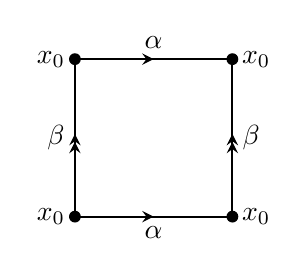
\begin{tikzpicture}
			\draw[thick, mid arrow] (0,0) to node[midway, below] {$\alpha$} (2,0);
			\draw[thick, mid arrow] (0,2) to node[midway, above] {$\alpha$} (2,2);
			\draw[thick, double mid arrow] (0,0) to node[midway, left] {$\beta$} (0,2);
			\draw[thick, double mid arrow] (2,0) to node[midway, right] {$\beta$} (2,2);
			\fill (0,0) circle (0.075);
			\fill (2,0) circle (0.075);
			\fill (0,2) circle (0.075);
			\fill (2,2) circle (0.075);
			\node[left] at (0,0) {$x_0$};
			\node[right] at (2,0) {$x_0$};
			\node[left] at (0,2) {$x_0$};
			\node[right] at (2,2) {$x_0$};
		\end{tikzpicture}
		\caption{Generators for $\pi_1(A, x_0)$}
		\label{fig:generating fundgrp of A}
	\end{figure}
	
	We are finally ready to conclude. Recall that by van Kampen's theorem, for any $x_0 \in A \cap B$,
	\[
	\pi_1(T, x_0) = \pi_1(A, x_0) *_{\pi_1(A \cap B, x_0)} \pi_1(B, x_0) \cong (F_{\alpha, \beta}) *_{\Z} 1.
	\]
	So $\pi_1(T, x_0)$ is generated by the loops $\alpha, \beta$, and there are no relations on $\alpha$ and $\beta$ except those obtained from amalgamating the copy of $\Z$ corresponding to $\pi_1(A \cap B, x_0)$. In particular, it suffices to identify the images of the generator of $\pi_1(A \cap B, x_0)$ in $F_{\alpha, \beta}$ and $1$. The image in $1$ is of course the identity element, whereas the image in the $F_{\alpha, \beta}$ is $\alpha\beta\alpha^{-1}\beta^{-1}$. To see this, recall that the generator is the loop that goes around $A \cap B$ once, and we can push this out to see it is the same element up to homotopy as the loop that goes around the boundary of the square once. This will first travel along $\alpha$, then $\beta$, then follow along the opposite copies of $\alpha$ and $\beta$ backwards, corresponding to the elements $\alpha^{-1}$ and $\beta^{-1}$. Hence the element we are identifying with the identity is $\alpha\beta\alpha^{-1}\beta^{-1}$. Thus,
	\[
	\pi_1(T, x_0) \cong \langle \alpha, \beta \mid \alpha\beta\alpha^{-1}\beta^{-1} = 1 \rangle.
	\]
	
	But this relation is equivalent to saying that the generators relate with one another, so this group is isomorphic to $\Z \times \Z$, which is the free abelian group on two generators. This can also be checked with an explicit isomorphism. Hence $\pi_1(T, x_0) \cong \Z \times \Z$. Luckily, this computation agrees with our original computation using the product!
\end{exa}

\begin{exa}
	Let's generalize the previous example slightly to compute the fundamental group of the genus-$2$ torus, which we will denote by $\Sigma_2$ (the orientable surface of genus $g$ is usually denoted by $\Sigma_g$). We can express $\Sigma_2$ as the quotient of another polygon, this time an octogon. This is probably not clear,  but it is true; the easiest way to see it is to cut the octogon in half as shown in \cref{fig:genus 2 octogon} and follow the gluing instructions to see that each half is a torus with a disk removed.
	
	\begin{figure}[h]
		\centering
		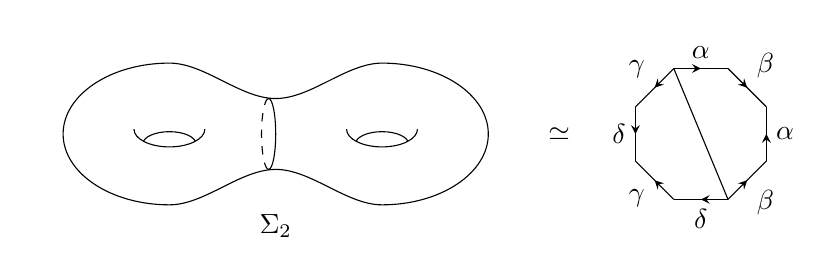
\begin{tikzpicture}[scale=0.9]
			\useasboundingbox (-2,-1.5) rectangle (9,1.5);
			\begin{scope}[shift={(7.5,0)}]
				\draw[mid arrow] (67.5:1) to node[midway, above right] {$\beta$} (22.5:1);
				\draw[mid arrow] (112.5:1) to node[midway, above] {$\alpha$} (67.5:1);
				\draw[mid arrow] (-22.5:1) to node[midway, right] {$\alpha$} (22.5:1);
				\draw[mid arrow] (-67.5:1) to node[midway, below right] {$\beta$} (-22.5:1);
				\draw[mid arrow] (112.5:1) to node[midway, above left] {$\gamma$} (157.5:1);
				\draw[mid arrow] (157.5:1) to node[midway, left] {$\delta$} (-157.5:1);
				\draw[mid arrow] (-67.5:1) to node[midway, below] {$\delta$} (-112.5:1);
				\draw[mid arrow] (-112.5:1) to node[midway, below left] {$\gamma$} (-157.5:1);
				\draw (112.5:1) -- (-67.5:1);
			\end{scope}
			\node at (5.5,0) {$\simeq$};
			\begin{scope}[shift={(0,0)}]
				\draw (-1.5,0) arc (180:90:1.5 and 1)
						.. controls +(0.5,0) and +(-0.5,0) .. (1.5,0.5)
						.. controls +(0.5,0) and +(-0.5,0) .. (3,1)
						arc (90:-90:1.5 and 1)
						.. controls +(-0.5,0) and +(0.5,0) .. (1.5,-0.5)
						.. controls +(-0.5,0) and +(0.5,0) .. (0,-1)
						arc (-90:-180:1.5 and 1);
				\begin{scope}
					\clip (-1,-1) rectangle (2,0.0675);
					\draw (0,0.0675) ellipse (0.5 and 0.25);
				\end{scope}
				\begin{scope}
					\clip (0,0.0675) ellipse (0.5 and 0.25);
					\draw (0,0.1725-0.3125) ellipse (0.375 and 0.1725);
				\end{scope}
				\begin{scope}
					\clip (2,-1) rectangle (4,0.0675);
					\draw (3,0.0675) ellipse (0.5 and 0.25);
				\end{scope}
				\begin{scope}
					\clip (3,0.0675) ellipse (0.5 and 0.25);
					\draw (3,0.1725-0.3125) ellipse (0.375 and 0.1725);
				\end{scope}
				\draw[dashed] (1.4,-0.5) arc (270:90:0.1 and 0.5);
				\draw (1.4,-0.5) arc (270:90:-0.1 and 0.5);
				\node[below] at (1.5,-1) {$\Sigma_2$};
			\end{scope}
		\end{tikzpicture}
		\caption{$\Sigma_2$ as the quotient of an octogon}
		\label{fig:genus 2 octogon}
	\end{figure}
	
	In similar fashion to what we did for the torus, we can cover the octogon with a neighborhood $A$ of the boundary and a disk $B$ in the center. Then as before,
	\[
	B \simeq \text{a point} \implies \pi_1(B, x_0) = 1 \qquad\text{and}\qquad A \cap B \simeq S^1 \implies \pi_1(A \cap B, x_0) \cong \Z
	\]
	where $\pi_1(A \cap B, x_0)$ is generated by a loop that goes around once. If we follow the same procedure for $A$, we obtain four circles that are all tangent at a point, corresponding to the four distinct loops in the boundary of the octogon. By a similar argument, this time covering the circles with four open sets (one neighborhood of each circle) and applying van Kampen's theorem, we find that $\pi_1(A, x_0) \simeq \Z * \Z * \Z * \Z$, which is isomorphic to the free product on four generators $\alpha, \beta, \gamma, \delta$ (as before, we have four generators and no relations). These generators are precisely the four loops in the boundary of the octogon.
	
	\begin{figure}[h]
		\centering
		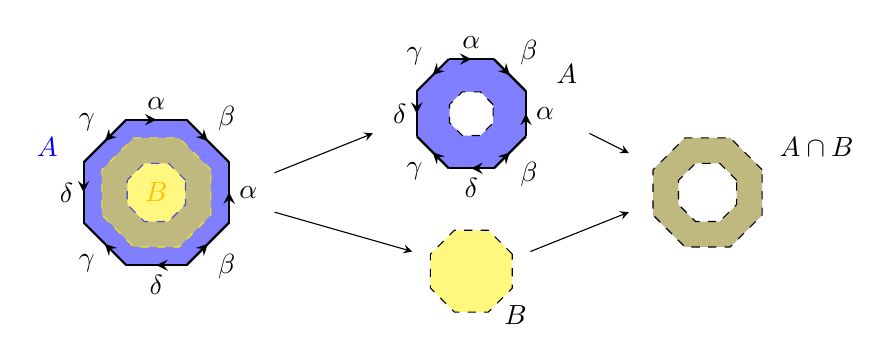
\begin{tikzpicture}
			\foreach \t in {0,...,7} \coordinate (a\t) at (\t*45 + 22.5:1);\foreach \t in {0,...,7} \coordinate (b\t) at (\t*45 + 22.5:0.75);
			\foreach \t in {0,...,7} \coordinate (c\t) at (\t*45 + 22.5:0.4);
			\fill[blue, opacity=0.5] (a0) -- (a1) -- (a2) -- (a3) -- (a4) -- (a5) -- (a6) -- (a7) -- cycle;
			\fill[white] (c0) -- (c1) -- (c2) -- (c3) -- (c4) -- (c5) -- (c6) -- (c7) -- cycle;
			\fill[yellow, opacity=0.5] (b0) -- (b1) -- (b2) -- (b3) -- (b4) -- (b5) -- (b6) -- (b7) -- cycle;
			\fill[white] (0.75,0.75) rectangle (1.25,1.25);
			\node[blue] at (157.5:1.5) {$A$};
			\node[orange!50!yellow] at (0,0) {$B$};
			\draw[dashed, yellow, opacity=0.9] (b0) -- (b1) -- (b2) -- (b3) -- (b4) -- (b5) -- (b6) -- (b7) -- cycle;
			\draw[dashed, blue, opacity=0.65] (c0) -- (c1) -- (c2) -- (c3) -- (c4) -- (c5) -- (c6) -- (c7) -- cycle;
			\draw[thick, mid arrow] (67.5:1) to node[midway, above right] {$\beta$} (22.5:1);
			\draw[thick, mid arrow] (112.5:1) to node[midway, above] {$\alpha$} (67.5:1);
			\draw[thick, mid arrow] (-22.5:1) to node[midway, right] {$\alpha$} (22.5:1);
			\draw[thick, mid arrow] (-67.5:1) to node[midway, below right] {$\beta$} (-22.5:1);
			\draw[thick, mid arrow] (112.5:1) to node[midway, above left] {$\gamma$} (157.5:1);
			\draw[thick, mid arrow] (157.5:1) to node[midway, left] {$\delta$} (-157.5:1);
			\draw[thick, mid arrow] (-67.5:1) to node[midway, below] {$\delta$} (-112.5:1);
			\draw[thick, mid arrow] (-112.5:1) to node[midway, below left] {$\gamma$} (-157.5:1);
			
			\draw[-stealth] (1.5,0.25) -- (2.75,0.75);
			\draw[-stealth] (1.5,-0.25) -- (3.25,-0.75);
			
			\begin{scope}[shift={(4,1)}, scale=0.75]
				\foreach \t in {0,...,7} \coordinate (a\t) at (\t*45 + 22.5:1);
				\foreach \t in {0,...,7} \coordinate (c\t) at (\t*45 + 22.5:0.4);
				\fill[blue, opacity=0.5] (a0) -- (a1) -- (a2) -- (a3) -- (a4) -- (a5) -- (a6) -- (a7) -- cycle;
				\fill[white] (c0) -- (c1) -- (c2) -- (c3) -- (c4) -- (c5) -- (c6) -- (c7) -- cycle;
				\draw[dashed] (c0) -- (c1) -- (c2) -- (c3) -- (c4) -- (c5) -- (c6) -- (c7) -- cycle;
				\draw[thick, mid arrow] (67.5:1) to node[midway, above right] {$\beta$} (22.5:1);
				\draw[thick, mid arrow] (112.5:1) to node[midway, above] {$\alpha$} (67.5:1);
				\draw[thick, mid arrow] (-22.5:1) to node[midway, right] {$\alpha$} (22.5:1);
				\draw[thick, mid arrow] (-67.5:1) to node[midway, below right] {$\beta$} (-22.5:1);
				\draw[thick, mid arrow] (112.5:1) to node[midway, above left] {$\gamma$} (157.5:1);
				\draw[thick, mid arrow] (157.5:1) to node[midway, left] {$\delta$} (-157.5:1);
				\draw[thick, mid arrow] (-67.5:1) to node[midway, below] {$\delta$} (-112.5:1);
				\draw[thick, mid arrow] (-112.5:1) to node[midway, below left] {$\gamma$} (-157.5:1);
				\node at (22.5:1.75) {$A$};
			\end{scope}
			
			\begin{scope}[shift={(4,-1)}, scale=0.75]
				\foreach \t in {0,...,7} \coordinate (b\t) at (\t*45 + 22.5:0.75);
				\fill[yellow, opacity=0.5] (b0) -- (b1) -- (b2) -- (b3) -- (b4) -- (b5) -- (b6) -- (b7) -- cycle;
				\draw[dashed] (b0) -- (b1) -- (b2) -- (b3) -- (b4) -- (b5) -- (b6) -- (b7) -- cycle;
				\node at (0.75,-0.75) {$B$};
			\end{scope}
			
			\draw[-stealth] (5.5,0.75) -- (6,0.5);
			\draw[-stealth] (4.75,-0.75) -- (6,-0.25);
			
			\begin{scope}[shift={(7,0)}]
				\foreach \t in {0,...,7} \coordinate (a\t) at (\t*45 + 22.5:1);\foreach \t in {0,...,7} \coordinate (b\t) at (\t*45 + 22.5:0.75);
				\foreach \t in {0,...,7} \coordinate (c\t) at (\t*45 + 22.5:0.4);
				\fill[blue, opacity=0.5] (b0) -- (b1) -- (b2) -- (b3) -- (b4) -- (b5) -- (b6) -- (b7) -- cycle;
				\fill[yellow, opacity=0.5] (b0) -- (b1) -- (b2) -- (b3) -- (b4) -- (b5) -- (b6) -- (b7) -- cycle;
				\fill[white] (c0) -- (c1) -- (c2) -- (c3) -- (c4) -- (c5) -- (c6) -- (c7) -- cycle;
				\draw[dashed] (b0) -- (b1) -- (b2) -- (b3) -- (b4) -- (b5) -- (b6) -- (b7) -- cycle;
				\draw[dashed] (c0) -- (c1) -- (c2) -- (c3) -- (c4) -- (c5) -- (c6) -- (c7) -- cycle;
				\node at (22.5:1.5) {$A \cap B$};
			\end{scope}
		\end{tikzpicture}
		\caption{Covering the octogon (really, $\Sigma_2$) with open sets}
		\label{fig:covering octogon}
	\end{figure}
	
	The amalgamation relations coming from $\pi_1(A \cap B, x_0)$ tell us to identify the loop that goes around the octogon once with the identity because it is trivial in $\pi_1(B, x_0)$. By pushing this loop out to the boundary (a homotopy) and following it around the boundary, we see that it is the element $\alpha\beta\alpha^{-1}\beta^{-1}\gamma\delta\gamma^{-1}\delta^{-1}$. Hence
	\[
	\pi_1(\Sigma_2, x_0) = \langle \alpha, \beta, \gamma, \delta \mid \alpha\beta\alpha^{-1}\beta^{-1}\gamma\delta\gamma^{-1}\delta^{-1} \rangle.
	\]
	Note that this is \emph{not} $\Z^4$; in particular, this relation does not even guarantee any of the generators commute with one another.
\end{exa}

\newpage
\section{Covering Spaces}
Covering spaces are extremely useful for understanding the fundamental group. For this section, we will assume that all spaces are path-connected and locally path-connected so that writing $\pi_1(X)$ has a clear meaning. We will still fix a basepoint when it is necessary to explicitly work with elements of $\pi_1$. The locally path-connected condition is needed for some point-set details that we won't go through.

\subsection{What is a Covering Space?}

\begin{defi}
	A map $p : \tilde X \to X$ is a \emph{covering map} if every point has an evenly covered neighborhood. A neighborhood $U$ is \emph{evenly covered} if $p^{-1}(U) = \bigsqcup_\alpha U_\alpha$ where $p$ takes each $U_\alpha$ homeomorphically to $U$.
\end{defi}

\begin{exa}
	$S^1$ is covered by $\R$ via the map $p : \theta \mapsto e^{2\pi i\theta}$, or equivalently via $x \mapsto [x \bmod{1}]$. We saw when computing $\pi_1(S^1)$. To see that this map is a covering map, note that for any $x \in S^1$, we can take a small open interval along $S^1$, whose preimage under $p$ will be a union of open intervals, which are all homeomorphic. Moreover, the open intervals will all have the same length and be translations by $1$ of each other, and are all taken homeomorphically by $p$ to the open interval along $S^1$.
	
	\begin{figure}[h]
		\centering
		\begin{tikzpicture}
			\draw[stealth-stealth] (-7,0) -- (7,0) node[below] {$\R$};
			
			\draw (0,-3.5) circle (1.5);
			\path (0,-3.5) -- +(225:1.5) node[below left] {$S^1$};
			\draw[ultra thick, blue] (0,-3.5)+(30:1.5) arc (30:150:1.5);
			\fill (0,-3.5)+(90:1.5) circle (0.075);
			
			\foreach \t in {-3,...,3} {
				\draw (2*\t,-0.1) -- (2*\t,0.1);
				\node[below] at (2*\t,-0.1) {$\t$};
				\draw[ultra thick, blue] (1/2+-1/3 + 2*\t,0) -- (1/2+1/3 + 2*\t,0);
				\fill (1/2+2*\t,0) circle (0.075);
			}
			
			\draw[-stealth] (0,-0.75) -- (0,-1.75) node[midway, right] {$\theta \mapsto e^{2\pi i\theta}$};
		\end{tikzpicture}
		\caption{$\R$ covers $S^1$}
		\label{fig:R cover S1}
	\end{figure}

\end{exa}

\begin{exa}
	The torus $\R^2/\Z^2$ is covered by $\R^2$ via the map $p : (x, y) \mapsto (x \bmod{1}, y \bmod{1})$. To see that this is a covering map, we think of the torus as a quotient of the square and take a small neighborhood of each point (for example, a ball with radius less than $1/2$); the preimage of the neighborhood will be many disjoint copies of the neighborhood, translated by elements of $\Z^2$. Each connected component is taken homeomorphically by $p$ to the neighborhood in the square; for non-boundary points of the square this is clear but for boundary points this requires some thought.
	
	\begin{figure}[h]
		\centering
		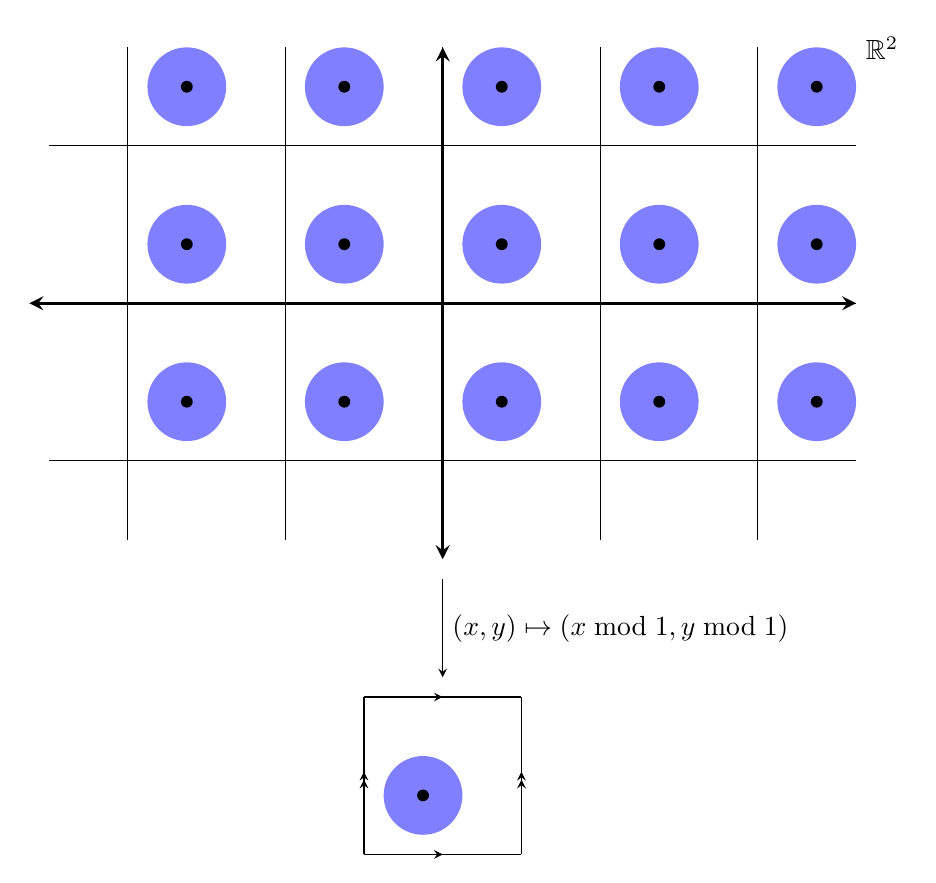
\begin{tikzpicture}
			\foreach \x in {-4,-2,...,4} \draw (\x,-3) -- (\x,3.25);
			\foreach \y in {-2,0,2} \draw (-5,\y) -- (5.25,\y);
			\draw[very thick, stealth-stealth] (-5.25,0) -- (5.25,0);
			\draw[very thick, stealth-stealth] (0,-3.25) -- (0,3.25);
			\node[right] at (5.25,3.24) {$\R^2$};
			
			\foreach \x in {-4,-2,...,4} {
				\foreach \y in {-2,0,2} {
					\begin{scope}[shift={(\x,\y)}]
						\fill[blue, opacity=0.5] (0.75,0.75) circle (0.5);
						\fill (0.75,0.75) circle (0.075);
					\end{scope}
				}
			}
			
			\draw[-stealth] (0,-3.5) -- (0,-4.75) node[midway, right] {$(x, y) \mapsto (x \bmod{1}, y \bmod{1})$};
			
			\begin{scope}[shift={(-1,-7)}]
				\draw[mid arrow,] (0,0) -- (2,0);
				\draw[mid arrow] (0,2) -- (2,2);
				\draw[double mid arrow] (0,0) -- (0,2);
				\draw[double mid arrow] (2,0) -- (2,2);
				
				\fill[blue, opacity=0.5] (0.75,0.75) circle (0.5);
				\fill (0.75,0.75) circle (0.075);
			\end{scope}
		\end{tikzpicture}
		\caption{$\R^2$ covers the torus}
		\label{fig:R2 cover torus}
	\end{figure}
	
	This construction can be generalized to show that $\R^n$ covers the $n$-torus $\R^n/\Z^n$.
\end{exa}

\begin{exa}
	The space consisting of two tangent circles, denoted $S^1 \vee S^1$, has many interesting covering spaces. One example is obtained by placing a copy of $S^1$ at each integer along $\R$. The covering map projects all the integer points to the tangent point of the two circles, so any sufficiently small neighborhood of the tangent point lifts homeomorphically to neighborhoods of the integers. A sufficiently small neighborhood of any other point lifts to either many neighborhoods in $\R$ or a neighborhood in each copy of $S^1$, depending on which circle the point is in. \cref{fig:cover S1 v S1} should clarify things visually.
	
	\begin{figure}[h]
		\centering
		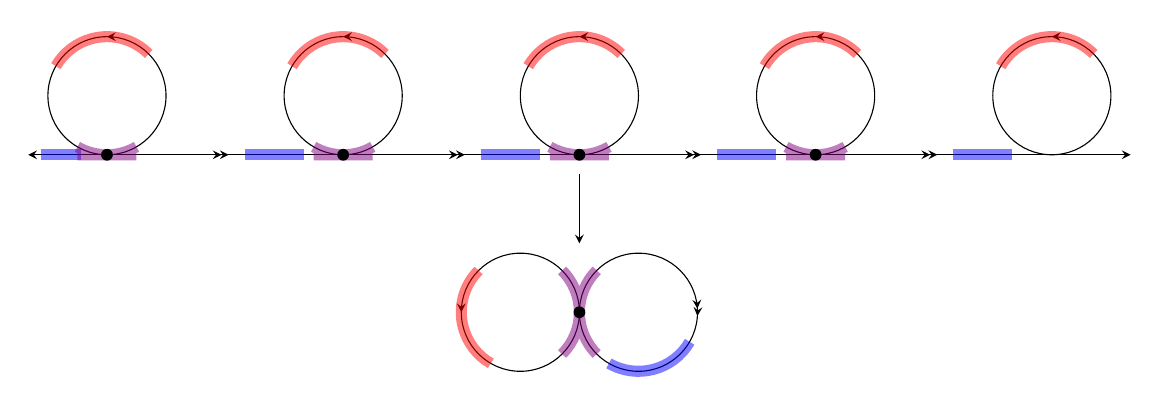
\begin{tikzpicture}
			\draw[stealth-] (-7,0) -- (-6,0);
			\draw[stealth-] (7,0) -- (6,0);
			\draw[line width=4, opacity=0.5, blue] (-8+7/6,0) -- (-8+5/3,0);
			\foreach \x in {-6,-3,...,3} {
				\draw[mid arrow] (\x,0) arc (-90:270:0.75);
				\draw[double mid arrow closeish] (\x,0) -- (\x+3,0);
				\draw[line width=4, opacity=0.5, red] (\x,0.75)+(45:0.75) arc(45:150:0.75);
				\draw[line width=4, opacity=0.5, blue] (\x+7/4,0) -- (\x+5/2,0);
				\draw[line width=4, opacity=0.5, violet] (\x-3/8,0) -- (\x+3/8,0) -- (\x,0) arc (270:240:0.75) arc (240:300:0.75);
				\fill (\x,0) circle (0.075);
			}
			\draw[mid arrow] (6,0) arc (-90:270:0.75);
			\draw[line width=4, opacity=0.5, red] (6,0.75)+(45:0.75) arc(45:150:0.75);
			
			\draw[-stealth] (0,-0.25) -- (0,-1.125);
			
			\draw[mid arrow] (0,-2) arc (0:360:0.75);
			\draw[double mid arrow close] (0,-2) arc (360:0:-0.75);
			\draw[line width=4, opacity=0.5, violet] (0,-2)
				arc (0:45:0.75)
				arc (45:-45:0.75)
				arc (-45:0:0.75)
				arc (360:315:-0.75)
				arc (315:405:-0.75);
			\draw[line width=4, opacity=0.5, blue] (0.75,-2)+(150:-0.75) arc (150:60:-0.75);
			\draw[line width=4, opacity=0.5, red] (-0.75,-2)+(135:0.75) arc (135:240:0.75);
			\fill (0,-2) circle (0.075);
		\end{tikzpicture}
		\caption{A cover of $S^1 \vee S^1$}
		\label{fig:cover S1 v S1}
	\end{figure}

\end{exa}

One of the most important results about covering spaces is the \emph{path lifting property}.

\begin{thm}\label{thm:path lifting}
	Consider a path $\gamma : I \to X$ starting at $x_0 \in X$ and a covering map $p : \tilde X \to X$ with a basepoint $\tilde x_0 \in p^{-1}(x_0)$. There is a unique path $\tilde\gamma : I \to \tilde X$ starting at $\tilde x_0$ such that $p \circ \tilde\gamma = \gamma$. Such a path $\tilde\gamma$ is called a \emph{lift} of $\gamma$.
\end{thm}

\begin{proof}
	Rigorously proving this theorem involves some technical point-set topology that we will not do in detail. Instead, here is the idea: we can construct a path $\tilde\gamma$ by starting at $\tilde x_0$. Since $\tilde x_0$ has a neighborhood which is mapped homeomorphically to a neighborhood of $x_0$, there is a unique way to lift $\gamma$ to $\tilde\gamma$ locally, i.e., in these homeomorphic neighborhoods. We can continue locally extending our path in this way, and by a compactness argument, finitely many extensions suffice. There are more details to worry about, but dealing with them is not sufficiently enlightening to write out here. Those interested can check Hatcher's book for the full proof.
\end{proof}

Since we have a nice result about paths in covering spaces, it is natural to expect a nice result about the fundamental groups of covering spaces. Indeed, we have such a result!

\begin{thm}
	If $p : \tilde X \to X$ is a covering map with $p(\tilde x_0) = x_0$, then the induced map $p_* : \pi_1(\tilde X, \tilde x_0) \to \pi_1(X, x_0)$ is injective.
\end{thm}

\begin{proof}
	If $p \circ \tilde\gamma_1 \simeq p \circ \tilde\gamma_2$ via a path-homotopy $H_t$, then each $H_t$ is a path in $X$ starting at $x_0$, which lifts uniquely to a path-homotopy $\tilde H_t$ from $\tilde\gamma_1$ to $\tilde\gamma_2$. This proves that if $p_*([\tilde\gamma_1]) = p_*([\tilde\gamma_2])$, then $[\tilde\gamma_1] = [\tilde\gamma_2]$, so $p_*$ is injective.
\end{proof}

This means we can identify $\pi_1(\tilde X, \tilde x_0)$ with a subgroup of $\pi_1(X, x_0)$. This is only the beginning of the results on fundamental groups of covers!

\subsection{Uniqueness of Associated covers}
Our motivation for this section will be to try to understand the statement ``the covering space associated to a subgroup of $\pi_1(X)$ is unique up to isomorphism.'' One important thing to understand is what we mean by ``isomorphism'' in the context (i.e., category) of covers. As always, an isomorphism is a structure-preserving bijection, which in this case means we need to preserve both the topological structure and the covering structure. This makes the following definition natural.

\begin{defi}
	Let $p_1 : \tilde X_1 \to X$ and $p_2 : \tilde X_2 \to X$ be covering maps. An \emph{isomorphism of covers} $f : \tilde X_1 \to \tilde X_2$ is a homeomorphism such that $p_2 \circ f = p_1$.
	\[
	\begin{tikzcd}
		\tilde X_1 \ar[rr, "f"] \ar[dr, "p_1"'] & & \tilde X_2 \ar[dl, "p_2"]\\
		& X
	\end{tikzcd}
	\]
	If we have distinguished basepoints $\tilde x_1 \in \tilde X_1$, $\tilde x_2 \in \tilde X_2$, and $x_0 \in X$ that agree with the covering structure (i.e., $p_1(\tilde x_1) = p_2(\tilde x_2) = x_0$), then $f$ is called \emph{basepoint-preserving} if $f(\tilde x_1) = f(\tilde x_2)$.
\end{defi}

We care about basepoint-preserving maps because basepoints are important for fundamental groups. Also note that if $f$ is only continuous (rather than a homeomorphism), then $f$ is called a \emph{map of covers}.

Our motivating result is that two covers of $X$ correspond to the same subgroup if and only if there is a basepoint-preserving isomorphism of covers between them. We can already prove the backward direction by taking $\pi_1$ of the relevant diagram for the isomorphism of covers. To prove the backward direction, we need two lemmas about maps to/between covers of $X$.

\begin{lem}\label{lem:map lift exists}
	If $p : \tilde X \to X$ is a cover and $f : Y \to X$, then there is a lift $\tilde f : Y \to \tilde X$ such that $p \circ \tilde f = f$ if and only if $f_*(\pi_1(Y)) \subseteq p_*(\pi_1(\tilde X))$. Moreover, such an $\tilde f$ is basepoint-preserving.
	\[
	\begin{tikzcd}
		& \tilde X \ar[d, "p"]\\
		Y \ar[r, "f"'] \ar[ur, dashed, "\tilde f"] & X
	\end{tikzcd}
	\]
\end{lem}

\begin{proof}
	($\impliedby$) If such an $\tilde f$ exists, then
	\[
	f_*(\pi_1(Y)) = p_*(\tilde f_*(\pi_1(Y))) \subseteq p_*(\pi_1(\tilde X)).
	\]
	
	($\implies$) Assuming $f_*(\pi_1(Y)) \subseteq p_*(\pi_1(\tilde X))$. We need to be more explicit, so fix basepoints $y_0 \in Y$, $x_0 \in X$, $\tilde x_0 \in \tilde X$ such that $f(y_0) = x_0$ and $p(\tilde x_0) = x_0$. Construct $\tilde f : Y \to \tilde X$ as follows: given $y \in Y$, let $\gamma$ be a path from $y_0$ to $y$; then $f \circ \gamma$ lifts uniquely to some path $\widetilde{f \circ \gamma}$ in $\tilde X$ starting at $\tilde x_0$. Define $\tilde f(y) = \widetilde{f \circ \gamma}(1)$; then by construction, $p \circ \tilde f = f$. We still need to show that this is doesn't depend on the choice of path in $Y$ and this is where we use the fact that $f_*(\pi_1(Y)) \subseteq p_*(\pi_1(\tilde X))$, but the construction is technical and not particularly interesting, so we will omit it (we similarly omit the proof that $f$ is continuous).
	
	To see that $\tilde f$ is basepoint-preserving, note that $f(y_0) = x_0$, so the path that gets lifted to $\tilde X$ is the constant path at $x_0$; this lifts to the constant path at $\tilde x_0$, so $\tilde f(y_0) = \tilde x_0$.
\end{proof}

Now that we have an existence result about maps to covers, we will also give a uniqueness result.

\begin{lem}\label{lem:map of covers unique}
	If $p_1 : \tilde X_1 \to X$ and $p_2 : \tilde X_2 \to X$ are covering maps, and $f, g : \tilde X_1 \to \tilde X_2$ are maps of covers, then $f = g$ if $f$ and $g$ agree at a single point.
\end{lem}

\begin{proof}
	This is a technical point-set result, so we omit the proof. Details are in Hatcher.
\end{proof}

We can now combine these results to prove the more difficult direction of our motivating results.

\begin{thm}
	If $p_1 : \tilde X_1 \to X$ and $p_2 : \tilde X_2 \to X$ are covering maps, then $(p_1)_*(\pi_1(\tilde X_1)) = (p_2)_*(\pi_1(\tilde X_2))$ if and only if there is a basepoint-preserving isomorphism of covers $f : \tilde X_1 \to \tilde X_2$ (the basepoints in question are basepoints for $\pi_1(X), \pi_1(\tilde X_1), \pi_1(\tilde X_2)$ that respect the coverin structure).
\end{thm}

\begin{proof}
	($\impliedby$) If such an $f$ exists, then $f_*$ is an isomorphism with inverse $(f^{-1})_*$, hence
	\[
	(p_1)_*(\pi_1(\tilde X_1)) = (p_2)_*(f_*(\pi_1(\tilde X_2))) = (p_2)_*(\pi_1(\tilde X_2)).
	\]
	
	($\implies$) By \cref{lem:map lift exists}, $p_1$ and $p_2$ lift to maps $\tilde p_1 : \tilde X_1 \to \tilde X_2$ and $\tilde p_2 : \tilde X_2 \to \tilde X_1$. The maps $\mathrm{id}_{\tilde X_1}$ and $\tilde p_2 \circ \tilde p_2$ are both maps of covers and they agree at the basepoints of $\tilde X_1, \tilde X_2$, so by \cref{lem:map of covers unique}, they are equal.
	\[
	\begin{tikzcd}
		\tilde X_1 \ar[drrr, "p_1"'] \ar[rr, dashed, "\tilde p_1"] \ar[rrrr, bend left, "\mathrm{id}_{\tilde X_1}"] && \tilde X_2 \ar[dr, "p_2"] \ar[rr, dashed, "\tilde p_2"] \ar[rrrr, bend left, "\mathrm{id}_{\tilde X_2}"] && \tilde X_1 \ar[dl, "p_1"'] \ar[rr, dashed, "\tilde p_1"] && \tilde X_2 \ar[dlll, "p_2"]\\[2em]
		&&& X
	\end{tikzcd}
	\]
	Note that this proof resembles the usual abstract nonsense proof of uniqueness of universal objects.
\end{proof}

\subsection{Existence of Covers}
Our motivation for this section will be to show that there is a cover associated with every subgroup of $\pi_1(X)$. We will do this by first constructing a cover corresponding to the trivial subgroup, then using this cover to construct covers for other subgroups. The subgroup associated to the trivial subgroup is called the \emph{universal cover}.

In order to construct the universal cover, we need a sufficiently nice space. More specifically, we need a path-conneccted, locally path-connected, semi-locally simply connected space. We know what the first two conditions mean; a space $X$ is \emph{semi-locally simply connected} if every point $x \in X$ has a neighborhood $U$ such that the inclusion $\pi_1(U) \hookrightarrow \pi_1(X)$ induced from the inclusion $U \hookrightarrow$ is the trivial map. Note that this does not mean that $\pi_1(U)$ is trivial, but if we look at loops in the larger space $X$, then every loop can be deformed to a point.

Assume henceforth that $X$ is path-connected, locally path-connected, and semi-locally simply connected. Let $x_0 \in X$ be a fixed basepoint. As a set, the univesal cover of $X$ is
\begin{align*}
	\tilde X &= \{ \text{paths in } X \text{ starting at } x_0 \text{, up to path-homotopy}\}\\
	&= \frac{\{ \gamma : I \to X \mid \gamma(0) = x_0 \}}{\simeq}.
\end{align*}
Note that $\gamma$ need not be a loop at $x_0$, despite the fact that we have frequently used $\gamma$ to denote loops at $x_0$.

To topologize $\tilde X$, we define a basis of open sets as follows: for each open, path connected $U$ with the induced map $\pi_1(U) \hookrightarrow \pi_1(X)$ and each $[\gamma] \in \tilde X$, define
\begin{align*}
	U_{[\gamma]} &= \{ \text{paths extending $\gamma$ ending in $U$} \}\\
	&= \{ \gamma * \delta \mid \delta(0) = \gamma(1) \text{ and } \delta(1) \in U \}.
\end{align*}
This is well-defined on path-homotopy classes because path-homotopic paths have the same endpoints. Our basis is then the collection of all such sets $U_{[\gamma]}$.

To make $\tilde X$ a covering space for $X$, define $p : \tilde X \to X$ by $p([\gamma]) = \gamma(1)$. This is well-defined on path-homotopy classes because path-homotopic paths have the same endpoints. This map is continuous because $p^{-1}(U) = \bigcup_{[\gamma] \in \tilde X} U_{[\gamma]}$ for path-connected, locally path-connected, open sets $U$ with $\pi_1(U) \hookrightarrow \pi_1(X)$ trivial and these sets form a basis of open sets for $X$. It is a covering map because $p$ restricts to homeomorphisms $U_{[\gamma]} \to U$, so the sets $U$ are evenly covered (this is where we use the semi-locally simply connected condition, to say that every point has such a neighborhood).

Note also that $p(\gamma_{x_0}) = x_0$. We will now prove some basic properties of $\tilde X$.

\begin{prop}\label{prop:universal path connected}
	$\tilde X$ is path-connected.
\end{prop}

\begin{proof}
	The proof is identical to showing that every path is homotopic (but not necessarily path-homotopic) to a constant path\footnote{This is where the perspective that a homotopy is a path in the space of functions is useful!}. Let $[\gamma] \in \tilde X$ and define $\gamma_t : I \to X$ by
	\[
	\gamma_t(s) = \begin{cases}
		\gamma(s) & \text{if } s \leq t\\
		\gamma(t) & \text{if } s \geq t.
	\end{cases}
	\]
	Then $\gamma_0 = \gamma_{x_0}$ and $\gamma_1 = \gamma$, so $t \mapsto [\gamma_t]$ is a path in $\tilde X$ from $[\gamma_{x_0}]$ to $[\gamma]$. Since every point in $\tilde X$ is connected by a path to $[\gamma_{x_0}]$, $\tilde X$ is path-connected.
\end{proof}

\begin{prop}
	$\pi_1(\tilde X, [\gamma_{x_0}])$ is trivial.
\end{prop}

\begin{proof}
	Let $\tilde\gamma$ be a loop in $\tilde X$ based at $[\gamma_{x_0}]$. Define a path $\gamma$ in $X$ by
	\[
	\gamma(t) = p(\tilde\gamma(t)) = \tilde\gamma(t)(1).
	\]
	Since $\tilde\gamma(0) = \tilde\gamma(1) = [\gamma_{x_0}]$, $\gamma$ is a loop in $X$ based at $x_0$. Also, we can view $[\gamma] \in \tilde X$, so let $t \mapsto [\gamma_t]$ be the path from $[\gamma_{x_0}]$ to $[\gamma]$ discussed in \cref{prop:universal path connected}. Then
	\[
	p([\gamma_t]) = \gamma_t(1) = \gamma(t) = \tilde\gamma(t)(1) = p(\tilde\gamma(t))
	\]
	by definition, so $t \mapsto [\gamma_t]$ and $\tilde\gamma$ are both lifts of $\gamma$ starting at $[\gamma_{x_0}]$. Hence $[\gamma_t] = [\tilde\gamma(t)]$ by the path-lifting property.
	
	Also, $\gamma_1 = \gamma$ by construction, so
	\[
	[\gamma] = [\gamma_1] = [\tilde\gamma(1)] = [\gamma_{x_0}]
	\]
	because $\tilde\gamma$ is a loop based at $[\gamma_{x_0}]$, so $p_*([\tilde\gamma]) = [\gamma] = [\gamma_{x_0}]$ by definition. So $p_*([\tilde\gamma]) = [\gamma_{x_0}]$ for all $[\tilde\gamma] \in \pi_1(\tilde X, [\gamma_{x_0}])$. Since $[\gamma_{x_0}]$ is the identity element of $\pi_1(X, x_0)$ and $p_*$ is injective, this proves $\pi_1(\tilde X, [\gamma_{x_0}])$ is trivial.
\end{proof}

Thus, we have the universal cover associated with the trivial subspace of $\pi_1(X)$. We now want to use $\tilde X$ to define a cover associated to other subgroups, which we will do by taking quotients.

Given a subgroup $H \leq \pi_1(X, x_0)$, we wantm to construct $p_H : \tilde X_H \to X$ such that $(p_H)_*(\pi_1(\tilde X_H)) = H$. Define $\tilde X_H = \tilde X/\sim$, where $\sim$ is the equivalence relation
\[
[\gamma_1] \sim [\gamma_2] \iff \big[ \gamma_1(1) = \gamma_2(1) \text{ and } [\gamma_1 * \bar\gamma_2] \in H \big].
\]
Note that $\gamma_1 * \bar\gamma_2$ is a loop in $X$ at $x_0$ because $\gamma_1$ and $\gamma_2$ are paths in $X$ starting at $x_0$. Because of the first condition for $\sim$, $p : \tilde X \to X$ factors through $\tilde X_H$ via a map $p_H : \tilde X_H \to X$, which is moreover a covering map.
\[
\begin{tikzcd}
	\tilde X \ar[d, "\pi"'] \ar[dd, bend left, "p"]\\
	\tilde X_H \ar[d, dashed, "p_H"']\\
	X
\end{tikzcd}
\]

\begin{prop}
	$(p_H)_*(\pi_1(\tilde X_H)) = H$.
\end{prop}

\begin{proof}
	Assume $\gamma$ is a loop in $X$ at $x_0$ and is lifted by $p_H$ to the path $\tilde\gamma : I \to \tilde X_H$ from $[\gamma_{x_0}]$ to $[\gamma]$ in $\tilde X_H$. Then $\tilde\gamma$ is a loop if and only if $\tilde\gamma(1) = [\gamma_{x_0}]$, but also $\tilde\gamma(1) = [\gamma]$, so $\tilde\gamma$ is a loop if and only if $[\gamma] \sim [\gamma_{x_0}]$. Thus, $[\gamma] \in \pi_1(X)$ is in the image of $(p_H)_*$ if and only if $[\gamma * \bar\gamma_{x_0}] \in H$, i.e., if $[\gamma] \in H$.
\end{proof}

\subsection{The Galois Correspondence}
So far, we have constructed a bijective correspondence between subgroups of $\pi_1(X)$ and isomorphism classes of covers of $X$. Also, as the subgroups get smaller, the covers get larger (e.g., the universal cover corresponds to the trivial subgroup; quotients of the universal cover correspond to larger subgroups), in the sense that there are projections from ``larger'' covers to ``smaller'' covers. This is called the \emph{Galois corresondence}, and the last thing we want to prove is that the intermediate projection maps always exist --- so far, we only know that we can project from the universal cover to its quotients.

This will justify the connection to Galois theory and the Galois correspondence for field extensions, since covers can be treated as extensions of the base space in an analgous way and we get the same correspondence with subgroups.

\begin{prop}
	If $p_1 : \tilde X_1 \to X$ and $p_2 : \tilde X_2 \to X$ are covering maps, then $p_1$ factors through $p_2$ if and only if $(p_1)_*(\pi_1(\tilde X_1)) \subseteq (p_2)_*(\pi_1(\tilde X_2))$. Moreover, if $p_1$ factors, it is by a covering map.
	\[
	\begin{tikzcd}
		\tilde X_1 \ar[d, dashed, "q"'] \ar[dd, bend left, "p_1"]\\
		\tilde X_1 \ar[d, "p_2"']\\
		X
	\end{tikzcd} \iff (p_1)_*(\pi_1(\tilde X_1)) \subseteq (p_2)_*(\pi_1(\tilde X_2))
	\]
\end{prop}

\begin{proof}
	($\implies$) If $p_1 = p_2 \circ q$ for some $q : \tilde X_1 \to \tilde X_2$, then
	\[
	(p_1)_*(\pi_1(\tilde X_1)) = (p_2)_*(q_*(\pi_1(\tilde X_1))) \subseteq (p_2)_*(\pi_1(\tilde X_2)).
	\]
	($\impliedby$) Assume $(p_1)_*(\pi_1(\tilde X_1)) \subseteq (p_2)_*(\pi_1(\tilde X_2))$. Note that each fiber of $p_1$ is in bijection with $(p_1)_*(\pi_1(\tilde X_1))$ because $(p_1)_*(\pi_1(\tilde X_1))$ acts by permutations on $p_1^{-1}(x)$ for all $x \in X$. Similarly, each fiber of $p_2$ is in bijection with $\pi_1(\tilde X_2)$, so we can use the map $(p_1)_*(\pi_1(\tilde X_1)) \hookrightarrow (p_2)_*(\pi_1(\tilde X_2))$ to define $q : p_1^{-1}(x) \to p_2^{-1}(x)$ for all $x \in X$. Since the fibers of $p_1$ cover $\tilde X_1$, this defines $q$. It is necessary to check that $q$ is continuous, but we will not do so here.
	
	Checking that $q$ is a covering map provided that it factors $p_1$ is tedious point-set topology that we will omit.
\end{proof}

This proves that we have an isomorphism of posets between isomorphism classes of covers of $X$ and subgroups of $\pi_1(X)$, where subgroups are partially ordered by containment and covers are partially ordered by existence of intermediate covering maps. The correspondence is given by taking the fundamental group of a cover and mapping it into $\pi_1(X)$ via the induced group homomorphism from the covering map, which we know is injective. This is the Galois correspondence for covering spaces!
\[
\begin{tikzcd}
	& & \tilde X \ar[dll, end anchor=north] \ar[dl, end anchor=north] \ar[d, end anchor=north] \ar[dr, end anchor=north] \ar[drr, end anchor=north]\\
	\vdots \ar[drr, start anchor=south] & \vdots \ar[dr, start anchor=south] & \vdots \ar[d, start anchor=south] & \vdots \ar[dl, start anchor=south] & \vdots \ar[dll, start anchor=south]\\
	& & X
\end{tikzcd}
\longleftrightarrow
\begin{tikzcd}
	& & 1 \ar[dll, end anchor=north] \ar[dl, end anchor=north] \ar[d, end anchor=north] \ar[dr, end anchor=north] \ar[drr, end anchor=north]\\
	\vdots \ar[drr, start anchor=south] & \vdots \ar[dr, start anchor=south] & \vdots \ar[d, start anchor=south] & \vdots \ar[dl, start anchor=south] & \vdots \ar[dll, start anchor=south]\\
	& & \pi_1(X)
\end{tikzcd}
\]

\subsection{Group Actions}
\subsubsection{$\pi_1$ Acting on Fibers and the Deck Group}
Recall our construction of the universal cover as the space of paths in $X$ starting at some fixed basepoint $x_0$, which is path-connected with trivial fundamental group. We then constructed $\tilde X_H$ corresponding to $H \leq \pi_1(X)$ by taking a quotient of $\tilde X$ where we identify $[\gamma]$ and $[\gamma']$ if $[\gamma * \bar\gamma'] \in H$. Generally, we like taking quotients by group actions rather than arbitrary relations, so it would be nice to find a group action that gives this quotient. Henceforth, we will assume all spaces are sufficiently nice, meaning path-connected and locally path-connected.

Given a covering map $p : \tilde X \to X$, we let $\pi_1(X, x_0)$ act on $p^{-1}(x_0)$ as follows: given $\tilde x \in p^{-1}(x_0)$ and $[\gamma] \in \pi_1(X, x_0)$, let $\tilde{\bar\gamma}$ be the lift of $\bar\gamma$ to $\tilde X$ starting at $\tilde x$. Then $[\gamma] \cdot \tilde x = \tilde{\bar\gamma}(1)$. This is well-defined on path-homotopy classes, and defines a group action of $\pi_1(X, x_0)$ on $p^{-1}(x_0)$ because taking the inverse of $\gamma$ allows us to preserve compositionality (the fact that we have to take the inverse comes from the fact that path composition is defined with the opposite convention as function composition: $\alpha * \beta$ does $\alpha$ first, then $\beta$).

To understand this action better, we will show that it is just the action of $\pi_1(X, x_0)$ on right cosets of $H := p_*(\pi_1(\tilde X, \tilde x_0))$ by right multiplication. First, we need to see that the points of $p^{-1}(x_0)$ correspond to right cosets of $H$. Such a bijection is given by $H[\gamma] \mapsto \tilde\gamma(1)$ where $\tilde\gamma$ is the lift of $\gamma$ starting at $\tilde x_0$. This is well-defined because if $[\alpha] \in \pi_1(\tilde X, \tilde x_0)$, then $\alpha$ is the lift of $p \circ \alpha$ starting at $\tilde x_0$, so for any right coset $H[\gamma]$, $H[(p \circ \alpha) * \gamma] = \alpha * \tilde\gamma(1) = \tilde\gamma(1)$. The inverse of this map is given by taking a preimage $\tilde x$ of $x_0$ and a path $\tilde \gamma$ from $\tilde x_0$ to $\tilde x$ (by path-connectedness) and mapping $\tilde x \mapsto H[p \circ \tilde\gamma]$. This is well-defined because if $\tilde\gamma, \tilde\gamma'$ are two different maps, then $[\tilde\gamma' * \bar{\tilde\gamma}] \in \pi_1(\tilde X, \tilde x_0)$, so $H[p \circ \gamma] = H[p \circ \gamma']$.

Now we can translate the action of $\pi_1(X, x_0)$ on $p^{-1}(x_0)$ to the action of $\pi_1(X, x_0)$ on right cosets of $H$. To do this, we just expand definitions: if $\tilde x \in p^{-1}(x_0)$, $\gamma_{\tilde x}$ is a path from $\tilde x_0$ to $\tilde x$, and $\gamma \in \pi_1(X, x_0)$, then
\[
[\gamma] \cdot \tilde x = \tilde{\bar\gamma}(1) = (\gamma_{\tilde x} * \tilde{\bar\gamma})(1) = [(p \circ \gamma_{\tilde x}) * \bar\gamma] \cdot \tilde x
\qquad\text{and}\qquad
[\gamma] \cdot H[p \circ \gamma_{\tilde x}] = H[(p \circ \gamma_{\tilde x}) * \bar\gamma].
\]

This is very important because if $H \trianglelefteq \pi_1(X, x_0)$ is a normal subgroup, then $\pi_1(X, x_0)/H$ acts on right-cosets of $H$ by right multiplication because this is just the quotient group acting on itself by right multiplication. Hence $\pi_1(X, x_0)/H$ acts on $p^{-1}(x_0)$. To understand the condition that $H \trianglelefteq \pi_1(X, x_0)$ and the quotient $\pi_1(X, x_0)/H$, we will introduce the \emph{deck group}.

Recall that an isomorphism of covering spaces is a homeomorphism that preserves covering structure.

\begin{defi}
	If $p : \tilde X \to X$ is a covering space, a covering space isomorphism $\tilde X \to \tilde X$ is called a \emph{deck transformation}. The group of deck transformations is the \emph{deck group}, which we will denote by $G(\tilde X)$.
\end{defi}

Note that a deck transformation lifts the covering map, and is therefore determined by the image of a single point. In particular, if we have a fixed basepoint $\tilde x_0 \in \tilde X$, then each element of $G(\tilde X)$ is determined by the image of $\tilde x_0$; since each element preserves the covering map, the image of $\tilde x_0$ is always in $p^{-1}(x_0)$ and so $G(\tilde X)$ is really a group of permutations of $p^{-1}(x_0)$.

\begin{defi}
	A covering space $p : \tilde X \to X$ is \emph{normal} when $G(\tilde X)$ acts transitively on $p^{-1}(x_0)$.
\end{defi}

\begin{prop}
	Let $p : \tilde X \to X$ be a covering space with $X, \tilde X$ path-connected and locally path-connected and $p(\tilde x_0) = x_0$. Set $H = p_*(\pi_1(\tilde X, \tilde x_0)) \leq \pi_1(X, x_0)$. Then
	\begin{enumerate}
		\item $\tilde X$ is normal if and only if $p_*(\pi_1(\tilde X, \tilde x_0))$ is normal in $\pi_1(X, x_0)$.
		\item $G(\tilde X) \cong N(H)/H$, where $N(H)$ is the normalizer of $H$ in $\pi_1(X, x_0)$, i.e., the largest subgroup of $\pi_1(X, x_0)$ in which $H$ is normal.
	\end{enumerate}
\end{prop}

\begin{proof}
	Omitted (see Hatcher).
\end{proof}

All in all, we have proved the following theorem.

\begin{thm}
	Let $p : \tilde X \to X$ be a covering space with $H = p_*(\pi_1(\tilde X, \tilde x_0)) \leq \pi_1(X, x_0)$. The following are equivalent:\begin{enumerate}
		\item $H$ is normal
		\item $\tilde X$ is a normal covering
		\item $\pi_1(X, x_0)/H$ acts transitively on $p^{-1}(x_0)$.
	\end{enumerate}
	In case these hold, $G(\tilde X) \cong \pi_1(X, x_0)/H$ and the action on $p^{-1}(x_0)$ is the same.\qed
\end{thm}

This action of $G(\tilde X)$ is really nice, and our next goal is to generalize it.

\subsubsection{Covering Space Actions}
\begin{defi}
	An action of a group $G$ on a space $X$ is a \emph{covering space action} if each $x \in X$ has a neighborhood $U$ such that all images $g \cdot U$ are disjoint.
\end{defi}

An important fact is that the deck group acts via a covering space action.

\begin{prop}
	If $p : \tilde X \to X$ is a covering space, then $G(\tilde X)$ acts via a covering space action.
\end{prop}

\begin{proof}
	Let $\tilde x \in \tilde X$ and let $U$ be an evenly covered neighborhood of $p(\tilde x)$. Then the slices of $p^{-1}(U)$ (i.e., the components on which $p$ restricts to a homeomorphism) are disjoint by definition and every deck transformation permutes them. Moreover, if $V$ is a slice and $g_1(V) \cap g_2(V) \neq \varnothing$, then $g_1$ and $g_2$ must agree at a point in $V$ because they must respect $p$. But deck maps are determined by the image of a point, so $g_1 = g_2$.
\end{proof}

In fact, the converse holds: every covering space action is the image of a deck group.

\begin{thm}
	If $G \curvearrowright X$ is a covering space action, then $X \twoheadrightarrow X/G$ is a normal covering map with deck group $G$.
\end{thm}

\begin{proof}
	Let $[x] \in X/G$. Then $x$ has a neighborhood $U$ in $X$ such that all images of $g \cdot U$ are disjoint; the image of $U$ in $X/G$ is evenly covered with slices $g \cdot U$. Since the multiplication maps $x \mapsto g \cdot x$ are deck transformations, $G$ is a subgroup of the deck group of $X$; moreover, if $f : X \to X$ is a deck transformation and $x \in X$, $f(x) = g \cdot x$ for some $g \in G$ because $f$ respects the covering map. Since deck maps are determined by the image of a point, it follows that every deck transformation is a multiplication map. Hence $G$ is the deck group of $X \twoheadrightarrow X/G$. Since the fiber of a point $[x] \in X/G$ is all the images $g \cdot x$ in $X$, this means that $X \twoheadrightarrow X/G$ is a normal covering space.
\end{proof}

\begin{cor}
	If $G \curvearrowright X$ is a covering space action, $X$ is path-connected and locally path-connected, and $p : X \twoheadrightarrow X/G$ is the natural covering map. Then
	\[
	\frac{\pi_1(X/G, [x])}{p_*(\pi_1(X, x))} \cong G.
	\]
\end{cor}

\begin{proof}
	This is our previous result characterizing the deck group of a normal covering space.
\end{proof}

A special case is the universal cover, when it exists, and we can now reinterpret our construction for the Galois correspondence in a more natural way. The deck group of $\tilde X$ is $\pi_1(X)/\pi_1(\tilde X) \cong \pi_1(X)$ because $\pi_1(\tilde X) = 1$. Therefore, $\pi_1(X)$ acts on $\tilde X$ via a covering space action, implying any subgroup of $\pi_1(X)$ acts via a covering space action. Finally, if $H \leq \pi_1(X)$, then (with sloppy notation that can only be interpreted one way)
\[
\pi_1(\tilde X/H) \cong \frac{\pi_1(\tilde X/H)}{\pi_1(\tilde X)} \cong H
\]
because $\pi_1(\tilde X) \cong 1$. This gives us the construction of intermediate covering spaces in the Galois correspondence in a much more natural way and makes it clear that if $H_1 \leq H_2 \leq \pi_1(X)$, then there is an intermediate cover $\tilde X/H_1 \twoheadrightarrow \tilde X/H_2$ (obtained by viewing $\tilde X/H_2 \cong (\tilde X/H_1)/H_2$).

\begin{thebibliography}{H}
	\bibitem[H]{H} Hatcher, Allen, \emph{Algebraic Topology}, Cambridge University Press, Cambridge, 2000. \href{https://pi.math.cornell.edu/~hatcher/AT/AT.pdf}{\texttt{https://pi.math.cornell.edu/~hatcher/AT/AT.pdf}}
\end{thebibliography}

\end{document}
